\documentclass[preprint,12pt]{elsarticle}

%% Options for Expert Systems with Applications:
%% \documentclass[preprint,12pt]{elsarticle} % Single-column format for peer-review
%% \documentclass[5p,twocolumn]{elsarticle}   % Final camera-ready two-column view

\journal{Expert Systems with Applications}

\usepackage[T1]{fontenc}
\usepackage{graphicx}
\usepackage{amsmath,amssymb}
\usepackage{booktabs}
\usepackage{makecell}
\usepackage{multirow}
\usepackage{array}
\usepackage{subcaption}
\usepackage[hyphens]{url}
\usepackage{hyperref}
\usepackage{tikz}
\usetikzlibrary{shapes.geometric,arrows.meta,positioning,calc,fit,backgrounds}

\hypersetup{
    colorlinks=true,
    linkcolor=blue,
    filecolor=magenta,      
    urlcolor=cyan,
    citecolor=blue,
}

\graphicspath{{./images/}}
\setlength\tabcolsep{6pt}
\raggedbottom

\begin{document}

\begin{frontmatter}

\title{SkelGym: Cross-Paradigm Kinematic Fusion and Dynamic Augmentation for 22-Class Gym Exercise Classification}

\author[1]{Xuan-Cuong Nguyen\corref{contrib}}
\ead{cuongnxde180528@fpt.edu.vn}

\author[1]{Nhat-Quang Truong\corref{cor1}\corref{contrib}}
\ead{quangtnde180544@fpt.edu.vn}

\author[1]{Quoc-Trinh Vo}
\ead{trinhvqde180556@fpt.edu.vn}

\cortext[cor1]{Corresponding author.}
\cortext[contrib]{These authors contributed equally to this work.}

\affiliation[1]{organization={FPT University},
            addressline={FPT City, Ngu Hanh Son},
            city={Da Nang},
            postcode={550000},
            country={Viet Nam}}

\begin{abstract}
Automated gym exercise recognition is critical for developing intelligent virtual personal trainer systems capable of monitoring workout execution, tracking training volume, and mitigating musculoskeletal injury risks. However, traditional RGB video approaches incur prohibitive computational costs, suffer from environmental background overfitting, and raise severe privacy concerns when streaming from home environments. We evaluate on a curated corpus of 1,024 in-the-wild videos spanning 22 fine-grained resistance exercises under strict video-level partitioning with no source-video overlap across train, validation, and test sets. We present \textbf{SkelGym}, a lightweight, privacy-aware intelligent exercise recognition framework operating exclusively on 3D skeletal coordinates extracted via monocular pose estimation. SkelGym introduces three core innovations: (1) a 117-dimensional \textit{Biomechanical Compound Representation} fusing relative 3D joint displacements with pairwise elevation and azimuth angles; (2) \textit{SkelGym-Aug}, an anatomically valid skeletal augmentation protocol preserving musculoskeletal constraints through bilateral sagittal reflection and gravitational yaw rotation; and (3) a cross-paradigm ensemble coupling a self-attention Transformer with a four-stream Adaptive Graph Convolutional Network via validation-calibrated SLSQP soft voting. SkelGym achieves \textbf{70.11\% window-level accuracy} and \textbf{77.68\% video-level consensus accuracy} (Macro F1: 0.7649) across 2,743 test windows from 233 held-out videos, with key architectural improvements verified statistically significant (McNemar $p < 10^{-11}$, Wilcoxon $p < 0.005$). With an ultra-low classifier inference latency of merely \textbf{0.42--4.33~ms} on host CPU (0.08--0.54~ms on CUDA, 1.11--9.91~ms on MPS; where single-model backbones execute in 0.42--1.16~ms and the full five-stream ensemble executes in 4.33~ms) per 32-frame window, SkelGym enables real-time, privacy-aware exercise recognition suitable for smart mirrors, mobile devices, and embedded gym displays. All source code, extracted skeletal representations, metadata, and pretrained checkpoints used for reproducibility are publicly available at \url{https://huggingface.co/Cuong2004/gym-exercise-classification}.
\end{abstract}

\begin{keyword}
Gym exercise classification \sep Skeleton-based action recognition \sep Adaptive Graph Convolutional Networks \sep Video Transformers \sep Biomechanical features \sep Real-time inference \sep Edge AI
\end{keyword}

\end{frontmatter}

\section{Introduction}

Regular physical resistance training and structured exercise play an essential role in improving cardiovascular health, metabolic longevity, muscular hypertrophy, and psychological well-being \cite{schoenfeld2010}. With modern demanding lifestyles and remote working environments, a rapidly growing population conducts workouts in home settings rather than commercial fitness centers. However, exercising without the supervision of certified strength and conditioning coaches frequently leads to improper kinetic execution, sub-optimal muscular recruitment, and elevated risks of acute or repetitive strain injuries (such as lumbar disc herniation, rotator cuff impingement, and patellar tendinopathy) \cite{riccio2024}. Consequently, there is an urgent demand for automated, intelligent virtual personal trainers capable of identifying exercise types in real-time, monitoring execution repetitions, and providing instantaneous biomechanical feedback.

Early computer vision frameworks for resistance exercise and action recognition were predominantly built upon appearance-based RGB video models, such as 2D/3D CNNs \cite{donahue2015,carreira2017,feichtenhofer2019} and spatiotemporal Vision Transformers (e.g., ViViT \cite{arnab2021}, TimeSformer \cite{bertasius2021}, Video Swin \cite{liu2022video}). While dense RGB representations capture visual cues such as gym equipment and barbells \cite{ng2015}, they exhibit three critical operational drawbacks in practical deployments.

First, dense spatio-temporal convolutions incur heavy computational overhead (often exceeding hundreds of GFLOPs), which precludes real-time execution on resource-constrained mobile phones, smart displays, or edge hardware. Second, appearance-based networks readily memorize spurious background correlations---including flooring patterns, studio lighting, bench upholstery, and athletic apparel---resulting in severe performance collapse when evaluated in novel domestic workout environments. Third, cloud-centric video architectures necessitate continuously transmitting unconstrained high-definition RGB video streams from private living spaces to remote servers, introducing network bandwidth bottlenecks and user privacy vulnerabilities.

\begin{figure*}[!t]
\centering
\resizebox{\textwidth}{!}{
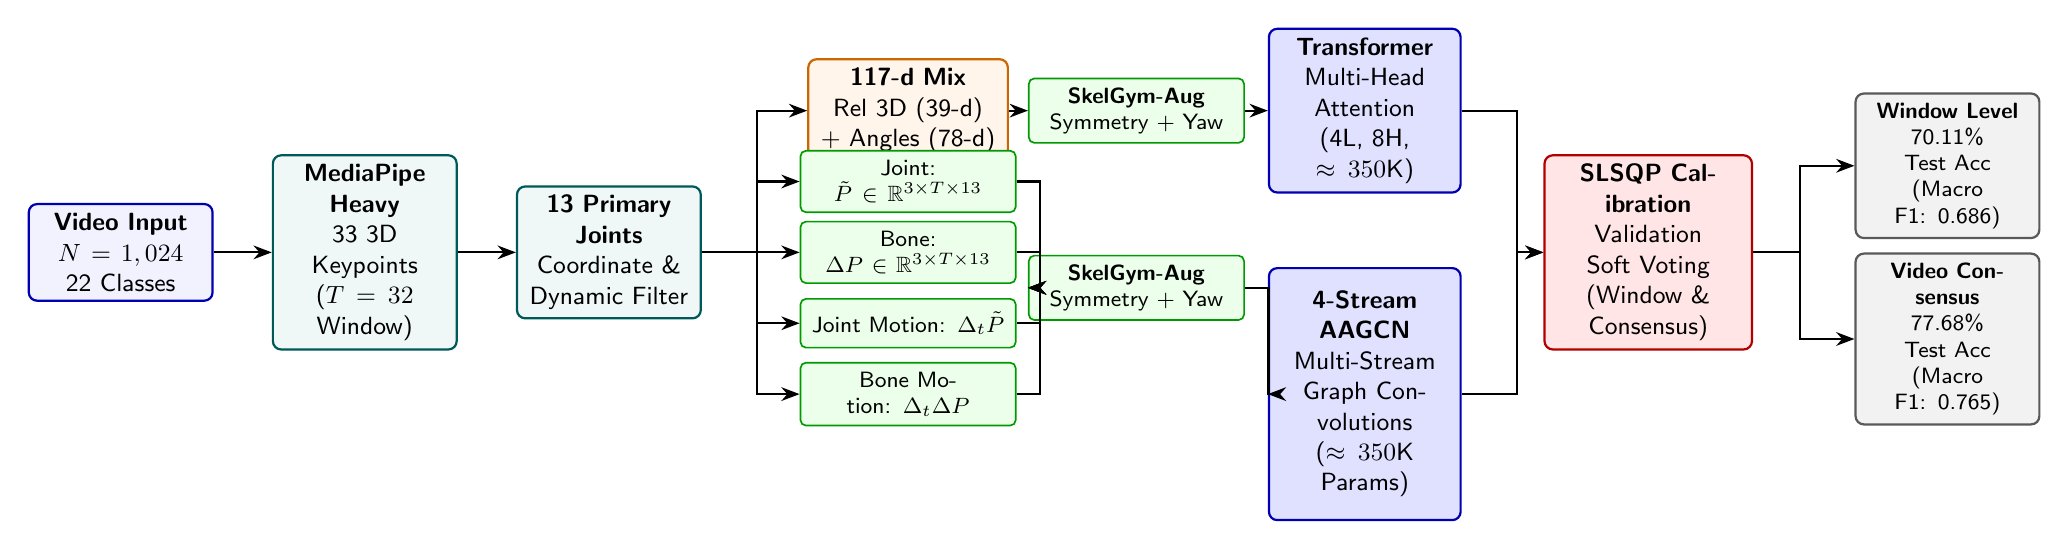
\begin{tikzpicture}[
    font=\sffamily\small,
    >=Stealth,
    block/.style={rectangle, draw=blue!70!black, fill=blue!5, rounded corners=3pt, text width=2.1cm, minimum height=1.1cm, align=center, line width=0.8pt},
    proc/.style={rectangle, draw=teal!70!black, fill=teal!6, rounded corners=3pt, text width=2.1cm, minimum height=1.1cm, align=center, line width=0.8pt},
    stream/.style={rectangle, draw=green!60!black, fill=green!8, rounded corners=2pt, text width=2.5cm, minimum height=0.62cm, align=center, line width=0.6pt, font=\sffamily\footnotesize},
    seqbox/.style={rectangle, draw=orange!80!black, fill=orange!8, rounded corners=3pt, text width=2.3cm, minimum height=1.1cm, align=center, line width=0.8pt},
    model/.style={rectangle, draw=blue!70!black, fill=blue!12, rounded corners=3pt, text width=2.2cm, minimum height=1.2cm, align=center, line width=0.8pt},
    modelaagcn/.style={rectangle, draw=blue!70!black, fill=blue!12, rounded corners=3pt, text width=2.2cm, minimum height=3.2cm, align=center, line width=0.8pt},
    fusion/.style={rectangle, draw=red!70!black, fill=red!10, rounded corners=3pt, text width=2.4cm, minimum height=1.3cm, align=center, line width=0.8pt},
    output/.style={rectangle, draw=gray!70!black, fill=gray!10, rounded corners=3pt, text width=2.1cm, minimum height=0.9cm, align=center, line width=0.8pt, font=\sffamily\footnotesize}
]

% Input & Feature Extraction
\node[block] (input) at (0, 0) {\textbf{Video Input}\\ $N=1,024$\\ 22 Classes};
\node[proc] (mp) at (3.1, 0) {\textbf{MediaPipe Heavy}\\ 33 3D Keypoints\\ ($T=32$ Window)};
\node[proc] (filter) at (6.2, 0) {\textbf{13 Primary Joints}\\ Coordinate \& Dynamic Filter};

% Top Branch: Transformer Mix
\node[seqbox] (comp) at (10.0, 1.8) {\textbf{117-d Mix}\\ Rel 3D (39-d)\\ + Angles (78-d)};
\node[stream] (aug1) at (12.9, 1.8) {\textbf{SkelGym-Aug}\\ Symmetry + Yaw};
\node[model] (trans) at (15.8, 1.8) {\textbf{Transformer}\\ Multi-Head Attention\\ (4L, 8H, $\approx 350$K)};

% Bottom Branch: Multi-Stream AAGCN
\node[stream] (joint) at (10.0, 0.9) {Joint: $\tilde{P} \in \mathbb{R}^{3 \times T \times 13}$};
\node[stream] (bone) at (10.0, 0.0) {Bone: $\Delta P \in \mathbb{R}^{3 \times T \times 13}$};
\node[stream] (jmot) at (10.0, -0.9) {Joint Motion: $\Delta_t \tilde{P}$};
\node[stream] (bmot) at (10.0, -1.8) {Bone Motion: $\Delta_t \Delta P$};

\node[stream] (aug2) at (12.9, -0.45) {\textbf{SkelGym-Aug}\\ Symmetry + Yaw};

\node[modelaagcn] (aagcn) at (15.8, -1.8) {\textbf{4-Stream AAGCN}\\ Multi-Stream\\ Graph Convolutions\\ ($\approx 350$K Params)};

% Fusion & Outputs
\node[fusion] (slsqp) at (19.4, 0) {\textbf{SLSQP Calibration}\\ Validation Soft Voting\\ (Window \& Consensus)};

\node[output] (out_win) at (23.2, 1.1) {\textbf{Window Level}\\ 70.11\% Test Acc\\ (Macro F1: 0.686)};
\node[output] (out_vid) at (23.2, -1.1) {\textbf{Video Consensus}\\ 77.68\% Test Acc\\ (Macro F1: 0.765)};

% Arrows
\draw[->, thick] (input) -- (mp);
\draw[->, thick] (mp) -- (filter);

\draw[->, thick] (filter.east) -- ++(0.7,0) |- (comp.west);
\draw[->, thick] (comp) -- (aug1);
\draw[->, thick] (aug1) -- (trans);

\draw[->, thick] (filter.east) -- ++(0.7,0) |- (joint.west);
\draw[->, thick] (filter.east) -- ++(0.7,0) |- (bone.west);
\draw[->, thick] (filter.east) -- ++(0.7,0) |- (jmot.west);
\draw[->, thick] (filter.east) -- ++(0.7,0) |- (bmot.west);

\draw[->, thick] (joint.east) -- ++(0.3,0) |- (aug2.west);
\draw[->, thick] (bone.east) -- ++(0.3,0) |- (aug2.west);
\draw[->, thick] (jmot.east) -- ++(0.3,0) |- (aug2.west);
\draw[->, thick] (bmot.east) -- ++(0.3,0) |- (aug2.west);

\draw[->, thick] (aug2.east) -- ++(0.3,0) |- (aagcn.west);

\draw[->, thick] (trans.east) -- ++(0.7,0) |- (slsqp.west);
\draw[->, thick] (aagcn.east) -- ++(0.7,0) |- (slsqp.west);

\draw[->, thick] (slsqp.east) -- ++(0.6,0) |- (out_win.west);
\draw[->, thick] (slsqp.east) -- ++(0.6,0) |- (out_vid.west);

\end{tikzpicture}
}
\caption{The proposed SkelGym architecture: an end-to-end cross-paradigm framework coupling self-attention sequence modeling with multi-stream adaptive graph convolutional networks via validation-calibrated weighted soft voting.}
\label{fig:pipeline_full}
\end{figure*}

Skeleton-based human action recognition offers an elegant solution to these challenges by abstracting human bodily movement into sparse, lightweight 3D keypoint coordinates. With real-time pose estimation frameworks such as Google MediaPipe \cite{chuankun2019,bazarevsky2020}, OpenPose \cite{cao2019}, and AlphaPose \cite{fang2022}, 3D skeletal tracking can be executed on commodity webcams and mobile chipsets at sub-millisecond latencies. However, translating skeletal tracking into accurate, multi-class gym exercise recognition introduces three fundamental scientific hurdles:

The first hurdle concerns biomechanical redundancy versus kinematic expressiveness. Resistance exercises frequently involve fine-grained differences in limb trajectories and joint angles, as demonstrated when distinguishing flat, incline, and decline bench presses, or differentiating conventional deadlifts from Romanian deadlifts. While exhaustive geometric angle formulations---such as computing all three-joint triplets---might capture these subtle distinctions, they incur a combinatorial explosion of features ($\binom{13}{3} = 286$), introducing dimensional multicollinearity, heavy computational overhead, and an acute risk of overfitting.

The second hurdle stems from physiologically invalid data augmentation. Conventional spatial transformations commonly employed in computer vision, such as random shearing, non-uniform affine scaling, or uncontrolled Gaussian jitter, distort biological joint limits and alter fixed anatomical bone lengths, synthesizing impossible body poses that corrupt network representation learning.

Finally, the third hurdle lies in achieving true cross-paradigm model complementarity while strictly preventing data contamination. Temporal sequence architectures (such as LSTMs \cite{hochreiter1997long,graves2005} and Transformers \cite{vaswani2017}) excel at modeling long-range phase transitions, whereas spatial-temporal graph convolutional networks (such as ST-GCN \cite{yan2018}, 2S-AGCN \cite{shi2019two}, and CTR-GCN \cite{chen2021channel}) explicitly exploit physical musculoskeletal topology. Prior works often combine these paradigms naively or tune ensemble fusion weights directly on test partitions, inducing optimistic reporting bias.

To systematically resolve these challenges, we introduce \textbf{SkelGym} (illustrated in Fig.~\ref{fig:pipeline_full}), an end-to-end intelligent exercise recognition system that transforms raw monocular video into actionable exercise labels through a fully automated pipeline: \textit{Video $\rightarrow$ MediaPipe 3D Skeleton $\rightarrow$ 117-d Biomechanical Representation $\rightarrow$ SkelGym-Aug $\rightarrow$ Cross-Paradigm Classifiers $\rightarrow$ SLSQP Ensemble $\rightarrow$ Video Consensus $\rightarrow$ Edge Deployment}. Specifically, this work provides four primary technical contributions:

\paragraph{C1: Biomechanical Compound Representation (117-d).} We design a compact kinematic descriptor unifying 3D relative joint coordinates (39-d) with pairwise elevation angles (78-d). This formulation provides both Euclidean metric awareness and scale-invariant directional orientation, resolving the severe multicollinearity and computational cost of combinatorial 3-joint angle triplets.

\paragraph{C2: Physiologically Grounded Data Augmentation (SkelGym-Aug).} We develop an on-the-fly skeletal augmentation protocol that respects human musculoskeletal constraints via bilateral sagittal reflection with exact angular permutations and gravitational 3D yaw rotations that preserve biological limb verticality \cite{ko2024augmentation}. Augmentation is confined exclusively to training forward passes, ensuring zero test-time data corruption.

\paragraph{C3: Custom Lightweight Architectures and Controlled Cross-Paradigm Benchmark.} Rather than fine-tuning massive pre-trained action recognition models, all backbones in SkelGym are lightweight networks ($\approx 350\text{K}$ parameters each) trained entirely from scratch, guaranteeing sub-millisecond edge classifier latencies. Under this controlled parameter footprint, we conduct an extensive comparative evaluation spanning recurrent networks, self-attention Transformers, and multi-stream adaptive graph convolutional networks.

\paragraph{C4: Validation-Calibrated Ensemble Optimization.} We establish a leakage-free SLSQP soft-voting formulation \cite{kraft1988,virtanen2020}, calibrating voting weights strictly on validation log-likelihoods for both window-level and temporal video consensus evaluations. SkelGym achieves 70.11\% window accuracy and 77.68\% video consensus accuracy across 22 resistance exercises with a classifier inference latency of 1.01~ms on Apple Silicon MPS per window. All code, datasets, and pre-trained checkpoints are publicly available for open science.

\section{Related Work}

\subsection{Skeletal Action Recognition}
Extracting human pose from monocular RGB video has matured rapidly with lightweight real-time estimators such as OpenPose \cite{cao2019}, AlphaPose \cite{fang2022}, and Google MediaPipe Pose \cite{chuankun2019,bazarevsky2020}. Early landmark-based action recognition utilized Recurrent Neural Networks (RNNs) and Long Short-Term Memory (LSTM) networks \cite{hochreiter1997long,graves2005,li2017} to model skeletal temporal dynamics. However, pure recurrent models treat skeletons as unorganized coordinate vectors, ignoring the inherent topological structure of the human musculoskeletal system.

To overcome this, Yan et al. \cite{yan2018} pioneered Spatial Temporal Graph Convolutional Networks (ST-GCN), constructing a spatio-temporal graph where human joints form vertices and physical bones form fixed spatial edges. Shi et al. \cite{shi2019two} introduced Two-Stream Adaptive Graph Convolutional Networks (2S-AGCN), parameterizing the adjacency matrix with learnable and data-driven components. Subsequent advances---including multi-stream AAGCN \cite{shi2020skeleton}, CTR-GCN \cite{chen2021channel}, InfoGCN \cite{chi2022infogcn}, HD-GCN \cite{lee2023hdgcn}, and SkateFormer \cite{zheng2024skateformer}---progressively integrated channel attention, information-theoretic representation learning, hierarchical graph decomposition, and partition-specific transformer attention. However, these modern architectures were predominantly tuned around large-scale benchmarks like NTU RGB+D (60/120 classes) with parameter footprints of $1.3\text{M}$--$5.2\text{M}$ and high GFLOP demands. In resistance exercise tracking, peripheral joints suffer severe occlusion by barbells and machine frames. SkelGym prunes the skeleton to $V=13$ load-bearing joints and designs custom lightweight backbones ($\approx 350\text{K}$ parameters per stream) trained from scratch, delivering real-time edge execution.

\subsection{Video Transformers and Attention in Kinematics}
Following the dominance of self-attention in NLP and computer vision (e.g., Vaswani et al. \cite{vaswani2017}, ViViT \cite{arnab2021}, TimeSformer \cite{bertasius2021}, Video Swin \cite{liu2022video}), transformers have been extended to skeletal motion (e.g., ST-TR \cite{plizzari2021sttr}). While transformers possess global receptive fields, they are data-hungry and prone to overfitting on limited skeletal training cohorts. We demonstrate that when fed with our 117-d Biomechanical Compound Representation and regularized by SkelGym-Aug, a compact 4-layer Transformer achieves competitive performance (68.65\% window accuracy), functioning as an ideal complement to graph convolutions.

\subsection{Skeletal Data Augmentation}
Data augmentation is critical for mitigating overfitting in skeleton-based recognition, particularly under limited training cohorts. Conventional spatial augmentations---such as random rotation, Gaussian coordinate jitter, random scaling, and temporal cropping---have been widely adopted \cite{yan2018,shi2020skeleton}. However, these generic transformations frequently violate anatomical constraints: non-uniform scaling distorts fixed bone lengths, unconstrained 3D rotations alter gravitational alignment, and random shearing synthesizes physiologically impossible postures. Ko et al. \cite{ko2024augmentation} systematically evaluated augmentation strategies for skeleton-based action recognition, demonstrating that carefully designed transformations yield significant accuracy improvements. In contrast to generic augmentations, SkelGym-Aug restricts transformations to the space of physiologically valid skeletal configurations through bilateral sagittal reflection (exact left-right joint and angular permutation) and gravitational yaw rotation (elevation-preserving $\mathrm{SO}(2)$ rotation about the vertical axis), ensuring all synthesized training samples represent anatomically plausible human postures.

\subsection{Ensemble Learning for Skeleton-Based Recognition}
Multi-stream fusion has emerged as a dominant paradigm in skeleton-based action recognition. Shi et al. \cite{shi2020skeleton} demonstrated that combining joint, bone, joint-motion, and bone-motion streams via late fusion substantially improves recognition accuracy by capturing complementary kinematic perspectives. However, existing multi-stream approaches typically employ either uniform averaging or manually tuned stream weights. Furthermore, when ensemble calibration involves test partition data---whether explicitly or implicitly through iterative hyperparameter sweeps---the resulting accuracy estimates suffer from optimistic reporting bias \cite{wolpert1992stacking}. SkelGym addresses both limitations through a principled SLSQP-based constrained optimization formulation \cite{kraft1988,virtanen2020} that calibrates stream voting weights exclusively on validation log-likelihoods, ensuring strictly held-out evaluation integrity.

\subsection{Fitness and Resistance Exercise Recognition}
Automated exercise tracking has attracted growing attention in sports science and ubiquitous computing. Riccio \cite{riccio2024} implemented real-time exercise classification and repetition counting using a BiLSTM over geometric joint angles. Ding et al. \cite{ding2022repcount} developed the RepCount benchmark for repetition counting in diverse fitness environments. Deyzel et al. \cite{deyzel2023} proposed one-shot skeleton-based recognition for strength and conditioning exercises on the SU-EMD dataset (5 exercises), revealing critical confusion between squats and deadlifts due to kinematic overlap. While general benchmarks (UCF101 \cite{soomro2012ucf101}, Kinetics-400 \cite{kay2017kinetics}) feature broad athletic activities, they lack fine-grained biomechanical resolution. Existing fitness datasets are either restricted to trivial 3--5 exercises or employ random temporal window splits that permit data leakage. In contrast, SkelGym benchmarks a demanding 22-class resistance exercise taxonomy under a strictly segregated video-level split protocol, advancing beyond laboratory-controlled settings to in-the-wild multi-camera gym environments.

\begin{figure*}[!t]
\centering
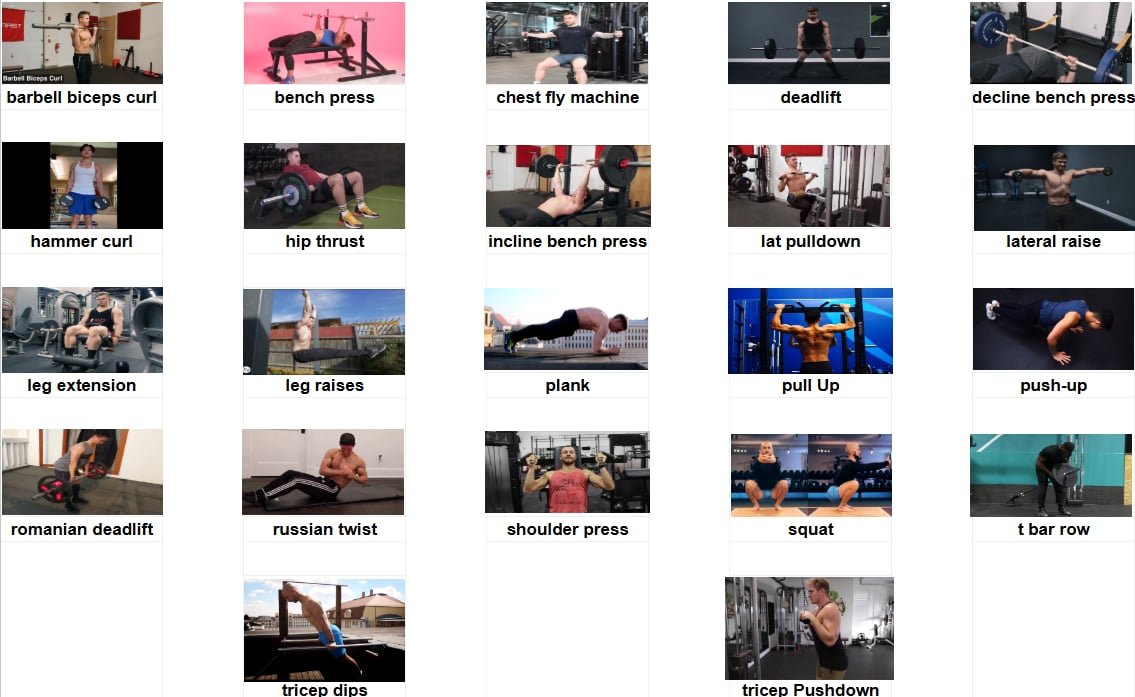
\includegraphics[width=0.88\textwidth]{images/Dataset.png}
\caption{Taxonomy and sample distributions across the 22 resistance exercises in the benchmark dataset.}
\label{fig:dataset_samples}
\end{figure*}

\section{Dataset and Experimental Protocol}

\subsection{Data Source, Provenance, and Ethical Compliance}
Our experimental corpus consists of 1,024 clean, un-shuffled video recordings across 22 resistance training exercises: \textit{barbell biceps curl, bench press, chest fly machine, deadlift, decline bench press, hammer curl, hip thrust, incline bench press, lat pulldown, lateral raise, leg extension, leg raises, plank, pull-up, push-up, Romanian deadlift, Russian twist, shoulder press, squat, t-bar row, tricep dips, and tricep pushdown} (Fig.~\ref{fig:dataset_samples}). To ensure high diversity in environmental backgrounds, camera angles, lighting conditions, and athlete anthropometry, the corpus unifies three distinct provenance streams: (1) \textit{public video repositories}, comprising 652 videos recovered from the open Workout/Exercise Video Dataset \cite{abdillah2023}; (2) \textit{curated online media}, including 103 high-definition clips collected from YouTube fitness channels, 65 clips from Pexels, and 76 clips from Freepik acquired under open research and stock licenses; and (3) \textit{author-recorded footage}, consisting of 128 supplementary videos captured by the authors in a gymnasium across all 22 exercise classes with two athletic models, employing both static tripod viewpoints and dynamic moving-camera angles to capture multi-perspective kinetic execution.

\begin{table*}[!t]
\centering
\caption{Key specifications, provenance breakdown, and capture characteristics of the GYMED exercise dataset.}
\label{tab:dataset_specs}
\resizebox{\textwidth}{!}{
\begin{tabular}{l l}
\toprule
\textbf{Specification / Characteristic} & \textbf{Value / Distribution} \\
\midrule
Total Videos / Total File Volume        & 1,024 unique video recordings / 10,225.37~MB ($\approx 10.2$~GB) \\
File Formats \& Video Encoding          & MP4 (964 videos, 94.1\%), MOV (60 videos, 5.9\%) / H.264 \\
Frame Rate \& Recording Duration        & 30 frames per second (FPS) / 20--30~s per recording \\
Trimmed Action Segments                 & 1,108 clean exercise segments (average 1.09 segments per video) \\
Number of Distinct Resolutions          & 33 resolutions (1280$\times$720: 385; 1920$\times$1080: 315; 720$\times$1280: 130; others: 194) \\
Exercise Taxonomy Coverage              & 22 fine-grained resistance exercise classes \\
Video Partitioning Ratio (6:2:2)        & Train: 580 (56.6\%), Validation: 208 (20.3\%), Test: 236 (23.1\%) \\
Action Segment Partitions               & Train: 639 (57.7\%), Validation: 210 (19.0\%), Test: 259 (23.3\%) \\
Temporal Windows ($T=32$ frames)        & Train: 13,136 ($S=16$), Validation: 2,075 ($S=32$), Test: 2,743 ($S=32$) \\
Multi-Source Data Provenance            & Abdillah (2023) \cite{abdillah2023}: 652; YouTube: 103; Pexels: 65; Freepik: 76; Authors: 128 \\
Subjects \& Ethical Compliance          & Informed consent under Declaration of Helsinki for recorded clips; diverse online athletes \\
Camera Dynamics \& Perspectives         & Static tripod and dynamic moving cameras; frontal, sagittal, oblique angles \\
Recording Environments                  & Commercial gymnasiums, domestic home workout spaces, outdoor fitness zones \\
\bottomrule
\end{tabular}
}
\end{table*}

\paragraph{Subject Statistics and Ethical Compliance.} To provide both high-precision kinematic reference baselines and expansive real-world diversity, the dataset incorporates two complementary subject cohorts. For the 128 self-recorded gymnasium videos, volunteer participants executed all 22 resistance movements under controlled multi-angle camera setups, providing kinematically disciplined execution benchmarks under formal written informed consent following the Declaration of Helsinki. For the remaining 896 web-sourced videos, recordings capture hundreds of diverse athletes spanning unconstrained body builds, athletic apparel, and training experience across international fitness facilities, home gyms, and outdoor parks. Crucially, the dataset does not annotate explicit participant demographic or gender identifiers, ensuring that model training and evaluation remain strictly posture-driven and invariant to demographic bias. Furthermore, the video-level partition ensures that 100\% of video clips and derived segments from any given recording session reside entirely within a single split, preventing subject or temporal leakage across train, validation, and test sets.

\paragraph{Source Statistics and Video Formats.} As summarized in Table~\ref{tab:dataset_specs}, the 1,024 video corpus totals 10,225.37~MB ($\approx 10.2$~GB) in storage, distributed between MP4 (964 videos, 94.1%) and MOV (60 videos, 5.9%) containers using H.264 compression. All videos operate at 30 frames per second. Video resolution was verified via \texttt{ffprobe}, encompassing 33 distinct resolutions dominated by standard high-definition formats: 1280$\times$720 (385 videos, 37.6%), 1920$\times$1080 (315 videos, 30.8%), and portrait mobile video 720$\times$1280 (130 videos, 12.7%), with 35 videos at 854$\times$480, 28 at 640$\times$360, 23 at 3840$\times$2160 (4K), and 108 videos distributed across 27 minor resolutions ($\le 20$ videos each).

\paragraph{Ethical Standards and Informed Consent.} For the 128 self-recorded videos, written informed consent was formally obtained from all participating human subjects prior to filming. The data recording protocol was conducted in strict adherence to institutional ethical standards and the Declaration of Helsinki. For data harvested from public online platforms, collection adhered strictly to platform Terms of Service and redistribution guidelines, gathering only publicly disseminated content without collecting private personal identifying information.

\paragraph{Data Licensing and Artifact Availability.} To respect the intellectual property and terms of external video hosting platforms (YouTube, Pexels, and Freepik), original raw third-party video recordings are not redistributed. Their original source identifiers, attribution information, and manual segmentation boundaries are retained within the metadata manifests. Instead, to guarantee 100\% scientific reproducibility, all derived scientific artifacts---including extracted 3D skeletal landmark coordinate tensors, manual action segmentation boundaries, preprocessed kinematic features, and metadata manifests---are publicly released under the Creative Commons Attribution 4.0 International license (CC BY 4.0). All neural network architectures, training routines, and pre-trained checkpoints are openly provided under the permissive MIT License at \url{https://huggingface.co/Cuong2004/gym-exercise-classification}.

\paragraph{Video Inclusion and Exclusion Criteria.} To ensure high-quality skeletal extraction and biomechanically meaningful training samples, we applied the following curation protocol. Videos were \textit{included} if they (i)~depicted a clearly identifiable single athlete performing one of the 22 target exercises, (ii)~were recorded at a frame rate of $\geq 25$~FPS, (iii)~contained at least one complete repetition cycle with visible concentric and eccentric phases, and (iv)~maintained sufficient camera framing such that hip and shoulder joints remained visible for $\geq 80\%$ of the active exercise duration. Conversely, videos were \textit{excluded} if they exhibited (a)~near-complete occlusion of both hip or both shoulder joints throughout the exercise segment (e.g., extreme close-up shots of isolated limbs), (b)~a native frame rate below 25~FPS (resulting in temporal aliasing during 30~FPS resampling), (c)~an active exercise duration shorter than one full repetition cycle ($< 32$ frames after trimming), or (d)~severe motion blur or compression artifacts rendering MediaPipe Pose landmark detection unreliable (landmark visibility confidence $< 0.3$ for $> 50\%$ of frames). This protocol yielded the final curated corpus of 1,024 videos described above.

\begin{figure*}[!t]
\centering
\begin{subfigure}[b]{0.48\textwidth}
    \centering
    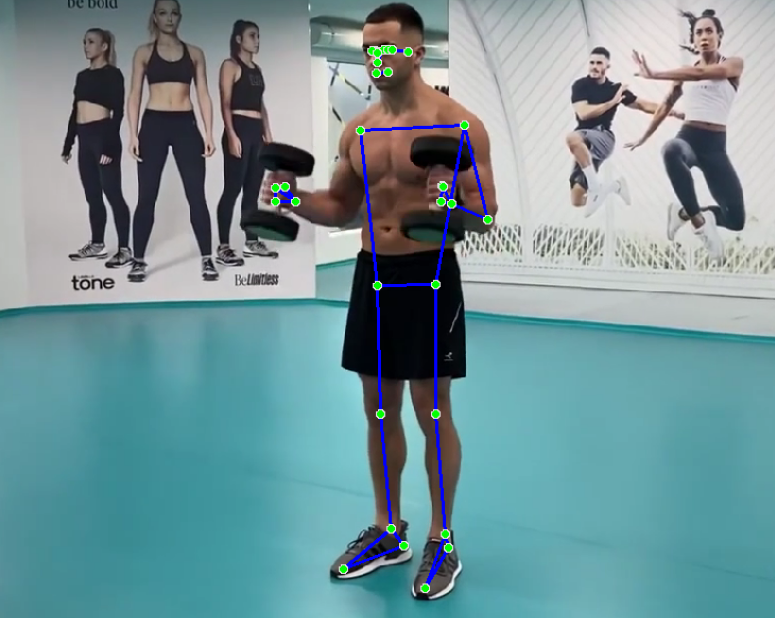
\includegraphics[width=\textwidth]{images/Mediapipe.png}
    \caption{Hammer curl}
    \label{fig:pose_hammer}
\end{subfigure}\hfill
\begin{subfigure}[b]{0.48\textwidth}
    \centering
    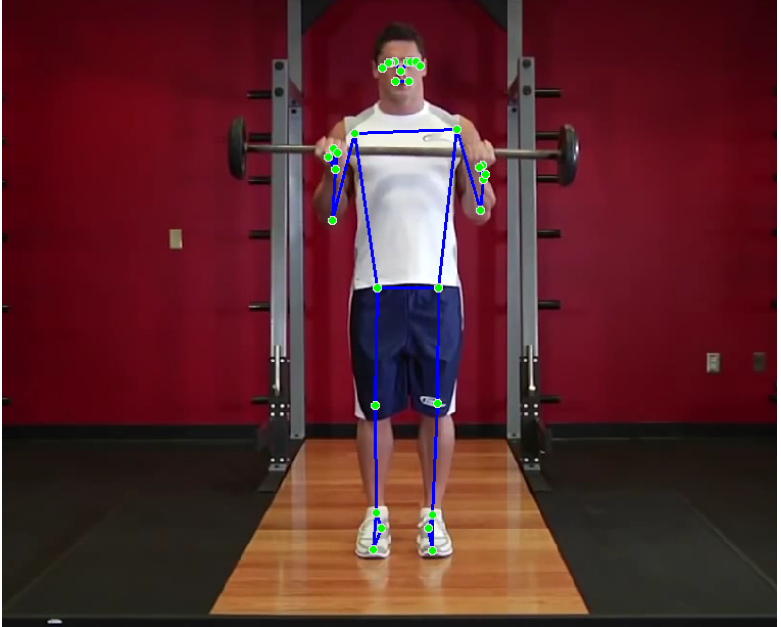
\includegraphics[width=\textwidth]{images/Mediapipe_2.png}
    \caption{Barbell biceps curl}
    \label{fig:pose_barbell}
\end{subfigure}
\caption{Full-body 3D pose landmark detection results across representative exercise video frames using Google MediaPipe Pose: (a) hammer curl and (b) barbell biceps curl.}
\label{fig:pose_detection}
\end{figure*}

\subsection{Action Trimming, Video-Level Partitioning, and Class Distribution}
Raw workout recordings frequently contain non-exercise transitional intervals, such as picking up barbells, adjusting bench pins, chalking hands, and resting. To eliminate noise, all 1,024 videos were manually verified and trimmed into action-only segments via timestamp boundary files (`.txt`), yielding 1,108 clean segments total (1.09 segments per video on average). 

\paragraph{Strict Video-Level Partitioning Protocol (No Source-Video Overlap Across Splits).} To ensure rigorous evaluation without data leakage, we enforce a strict video-level partition in a 6:2:2 ratio. Our data processing follows a strictly segregated 4-step pipeline: (1) \textit{Video-Level Isolation}: Raw video recordings are partitioned strictly by source video file into Train ($N=580$), Validation ($N=208$), and Test ($N=236$) sets, ensuring no video file or recording session spans across partitions. (2) \textit{Independent Landmark Extraction}: Monocular 3D skeletal landmarks are extracted independently per video file using Google MediaPipe Pose without inter-video context. (3) \textit{Within-Video Sliding Window Segmentation}: Temporal windows ($T = 32$ frames) are extracted strictly within individual trimmed action boundaries: $S = 16$ frames (50\% overlap) for Train (13,136 windows) to provide dense temporal coverage, and $S = 32$ frames (non-overlapping) for Validation (2,075 windows) and Test (2,743 windows across 233 videos with valid segments $\ge 32$ frames). No sliding window is permitted to cross video or segment boundaries. (4) \textit{Independent Window Normalization}: Spatial centering (subtracting mid-hip) and torso-scale normalization are calculated strictly on each individual window or frame, avoiding any dataset-wide parameter leakage. This strict protocol guarantees zero source-video overlap, zero temporal window leakage, and zero cross-partition parameter leakage. Because web-sourced exercise recordings lack explicit biometric subject identifiers, this strict video-level partition guarantees that all sub-clips, temporal windows, and repetitions from any single recording session reside exclusively within a single partition (Train, Validation, or Test), eliminating both temporal sequence leakage and intra-session environment memorization.

\begin{table*}[!t]
\centering
\caption{Video and action segment distributions across the 22 resistance training exercises by split (Train / Val / Test).}
\label{tab:class_distribution}
\resizebox{\textwidth}{!}{
\begin{tabular}{l c c | l c c}
\toprule
\textbf{Exercise Class} & \textbf{Videos (Tr/Va/Te)} & \textbf{Segments (Tr/Va/Te)} & \textbf{Exercise Class} & \textbf{Videos (Tr/Va/Te)} & \textbf{Segments (Tr/Va/Te)} \\
\midrule
Barbell biceps curl     & 52 / 18 / 14 & 53 / 18 / 14 & Leg raises            & 15 /  6 / 11 & 15 /  6 / 11 \\
Bench press             & 51 / 18 / 15 & 51 / 18 / 15 & Plank                 &  5 /  2 /  2 &  5 /  2 /  2 \\
Chest fly machine       & 28 /  9 /  8 & 29 /  9 /  8 & Pull-up               & 31 / 11 / 10 & 31 / 11 / 10 \\
Deadlift                & 30 / 10 / 10 & 30 / 10 / 10 & Push-up               & 40 / 14 / 12 & 43 / 14 / 14 \\
Decline bench press     & 18 /  5 /  9 & 29 /  5 / 10 & Romanian deadlift     & 12 /  6 /  6 & 13 /  6 /  8 \\
Hammer curl             & 24 /  8 / 14 & 28 /  8 / 14 & Russian twist         & 15 /  6 /  6 & 19 /  6 /  6 \\
Hip thrust              & 14 /  6 /  9 & 19 /  6 / 15 & Shoulder press        & 27 / 10 / 13 & 28 / 10 / 14 \\
Incline bench press     & 27 / 10 /  9 & 27 / 10 /  9 & Squat                 & 24 / 10 / 15 & 27 / 11 / 17 \\
Lat pulldown            & 42 / 15 / 14 & 42 / 15 / 15 & T-bar row             & 15 /  4 / 10 & 17 /  4 / 10 \\
Lateral raise           & 24 /  8 / 15 & 24 /  8 / 15 & Tricep pushdown       & 39 / 14 / 12 & 39 / 14 / 12 \\
Leg extension           & 22 /  9 / 13 & 27 /  9 / 13 & Tricep dips           & 25 /  9 /  9 & 43 / 10 / 25 \\
\midrule
\multicolumn{3}{l|}{\textbf{Total Videos:} 580 / 208 / 236 ($N=1,024$)} & \multicolumn{3}{l}{\textbf{Total Segments:} 639 / 210 / 259 ($N=1,108$)} \\
\bottomrule
\end{tabular}
}
\end{table*}

\paragraph{Class Imbalance and Metric Selection.} Table~\ref{tab:class_distribution} details the distribution of videos and action segments across all 22 classes. As shown, natural gym workout data exhibits significant class imbalance: highly popular compound movements such as \textit{barbell biceps curl} ($N=84$ videos) and \textit{bench press} ($N=84$ videos) possess large sample representations, whereas specialized exercises such as \textit{plank} ($N=9$ videos total: 5 train, 2 val, 2 test) are relatively scarce. To prevent models from artificially inflating overall accuracy by predicting majority classes, we adopt \textbf{Macro-averaged F1 score} alongside Accuracy as the primary evaluation benchmark.

\paragraph{Data and Code Availability.} To promote open science and persistent reproducibility, all extracted 3D pose landmark sequences (in JSON, NPY, and HDF5 tensor formats), action segmentations (\texttt{.txt}), partition manifests, and Python code are publicly hosted on Hugging Face Hub at \url{https://huggingface.co/Cuong2004/gym-exercise-classification}. Distributing pre-extracted coordinates circumvents vulnerability to third-party URL link rot common in video scraping, protects athlete privacy, and ensures permanent deterministic reproducibility. Raw third-party internet video recordings are withheld in adherence to platform Terms of Service, while the 128 author-recorded gymnasium clips and complete skeletal tensors are freely accessible for non-commercial academic research (see Appendix~\ref{app:open_science}). \textbf{Licensing:} The extracted 3D landmark coordinate tensors (NPY, JSON, HDF5), action segmentation boundaries, and partition manifests are released under the \textbf{Creative Commons Attribution 4.0 International (CC~BY~4.0)} license. All source code, training scripts, evaluation pipelines, and configuration files are released under the \textbf{MIT License}.

\subsection{Landmark Extraction and Anatomical Joint Selection}
Every video frame is processed through Google MediaPipe Pose Heavy (complexity level 2) \cite{chuankun2019,bazarevsky2020}, extracting 33 full-body 3D landmarks $(x_i, y_i, z_i, \text{vis}_i)$ normalized relative to bounding box and depth dimensions, as illustrated on representative workout frames in Fig.~\ref{fig:pose_detection}. Because facial landmarks and fine-grained finger points contribute negligible kinetic leverage to compound resistance exercises while introducing tracking jitter, we filter the skeleton to $V=13$ major anatomical joints (detailed in Table~\ref{tab:landmark_mapping}): nose (origin anchor), left/right shoulders, left/right elbows, left/right wrists, left/right hips, left/right knees, and left/right ankles.

\section{Proposed Methodology}
\label{sec:methodology}

The overall architectural workflow of \textbf{SkelGym} is illustrated in Fig.~\ref{fig:pipeline_full}, while Fig.~\ref{fig:feat_extraction_pipeline} details the underlying biomechanical feature extraction and kinematic tensor decomposition. Below, we formally derive each mathematical component of our framework.

\begin{figure}[!t]
\centering
\resizebox{\textwidth}{!}{
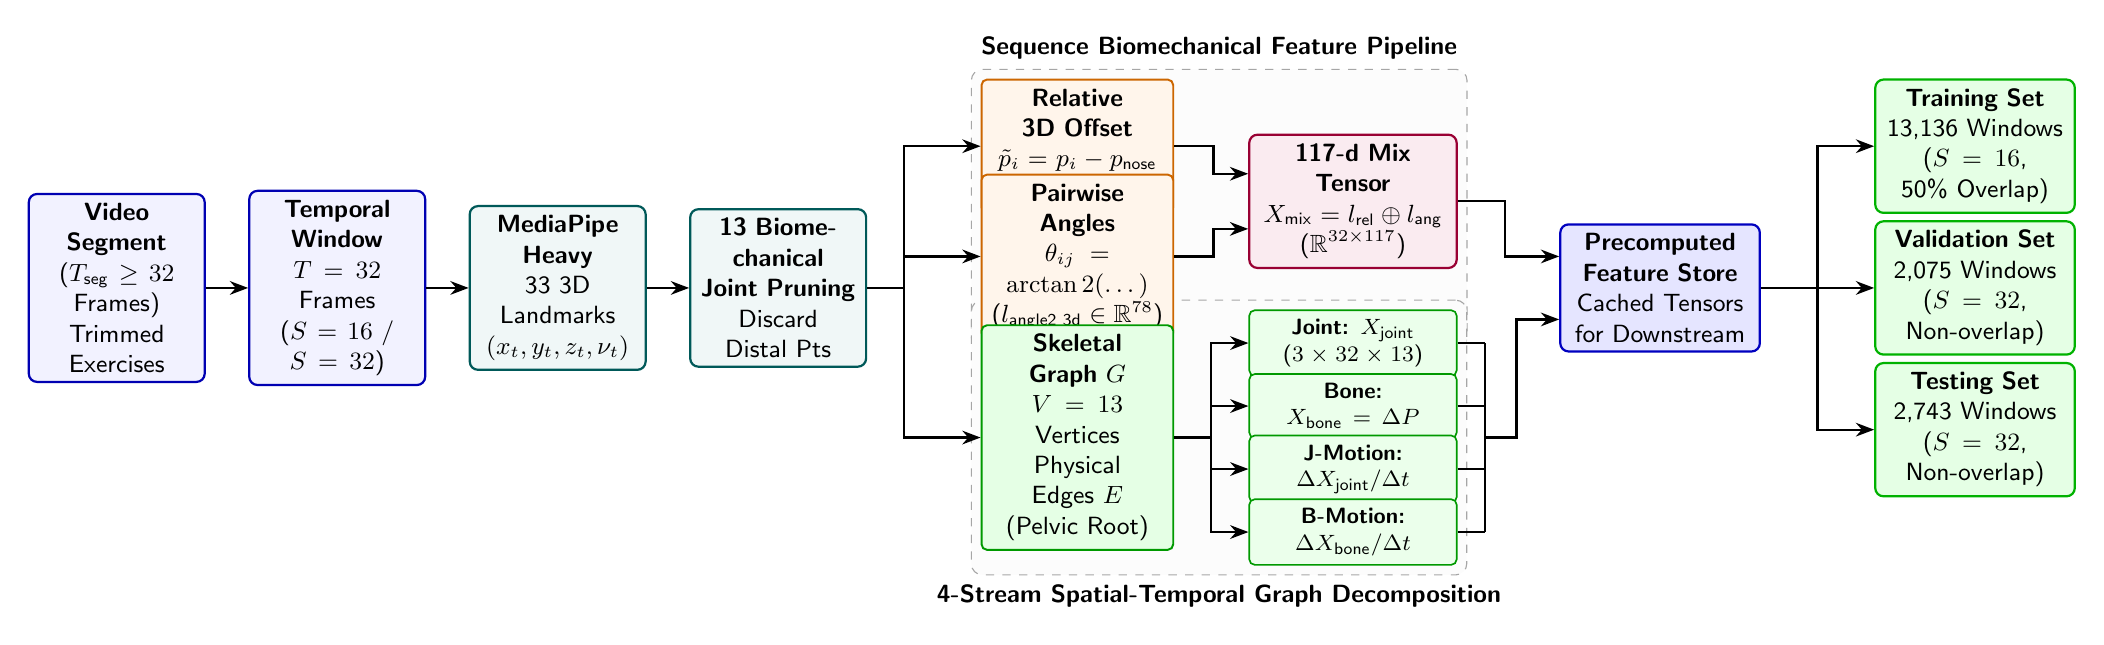
\begin{tikzpicture}[
    font=\sffamily\small,
    >=Stealth,
    block/.style={rectangle, draw=blue!70!black, fill=blue!5, rounded corners=3pt, text width=2.0cm, minimum height=1.1cm, align=center, line width=0.8pt},
    proc/.style={rectangle, draw=teal!70!black, fill=teal!6, rounded corners=3pt, text width=2.0cm, minimum height=1.1cm, align=center, line width=0.8pt},
    subproc/.style={rectangle, draw=orange!80!black, fill=orange!8, rounded corners=2pt, text width=2.2cm, minimum height=0.95cm, align=center, line width=0.7pt},
    tensor/.style={rectangle, draw=purple!80!black, fill=purple!8, rounded corners=3pt, text width=2.4cm, minimum height=1.3cm, align=center, line width=0.8pt},
    stream/.style={rectangle, draw=green!60!black, fill=green!8, rounded corners=2pt, text width=2.4cm, minimum height=0.58cm, align=center, line width=0.6pt, font=\sffamily\footnotesize},
    archive/.style={rectangle, draw=blue!75!black, fill=blue!10, rounded corners=3pt, text width=2.3cm, minimum height=1.5cm, align=center, line width=0.8pt},
    data/.style={rectangle, draw=green!70!black, fill=green!10, rounded corners=3pt, text width=2.3cm, minimum height=1.0cm, align=center, line width=0.8pt},
    group/.style={draw=black!35, dashed, rounded corners=4pt, fill=gray!2}
]

% Stage 1: Input and Pose Extraction (0.8cm clear gaps)
\node[block] (raw) at (0, 0) {\textbf{Video Segment}\\ ($T_{\text{seg}} \ge 32$ Frames)\\ Trimmed Exercises};
\node[block] (win) at (2.8, 0) {\textbf{Temporal Window}\\ $T=32$ Frames\\ ($S=16$ / $S=32$)};
\node[proc] (mp) at (5.6, 0) {\textbf{MediaPipe Heavy}\\ 33 3D Landmarks\\ $(x_t, y_t, z_t, \nu_t)$};
\node[proc] (filter) at (8.4, 0) {\textbf{13 Biomechanical}\\ \textbf{Joint Pruning}\\ Discard Distal Pts};

% Stage 2A: Upper Track - Sequence Feature Mix (y = 1.1)
\node[subproc] (rel) at (12.2, 1.8) {\textbf{Relative 3D Offset}\\ $\tilde{p}_i = p_i - p_{\text{nose}}$\\ ($l_{\text{rel\_3d}} \in \mathbb{R}^{39}$)};
\node[subproc] (ang) at (12.2, 0.4) {\textbf{Pairwise Angles}\\ $\theta_{ij} = \arctan2(\dots)$\\ ($l_{\text{angle2\_3d}} \in \mathbb{R}^{78}$)};
\node[tensor] (xmix) at (15.7, 1.1) {\textbf{117-d Mix Tensor}\\ $X_{\text{mix}} = l_{\text{rel}} \oplus l_{\text{ang}}$\\ ($\mathbb{R}^{32 \times 117}$)};

% Stage 2B: Lower Track - Multi-Stream Graph Kinematics (y = -1.9)
\node[subproc, fill=green!10, draw=green!60!black, minimum height=2.2cm, font=\sffamily\small] (graph) at (12.2, -1.9) {\textbf{Skeletal Graph $G$}\\ $V=13$ Vertices\\ Physical Edges $E$\\ (Pelvic Root)};

\node[stream] (g1) at (15.7, -0.7) {\textbf{Joint:} $X_{\text{joint}}$ ($3 \times 32 \times 13$)};
\node[stream] (g2) at (15.7, -1.5) {\textbf{Bone:} $X_{\text{bone}} = \Delta P$};
\node[stream] (g3) at (15.7, -2.3) {\textbf{J-Motion:} $\Delta X_{\text{joint}} / \Delta t$};
\node[stream] (g4) at (15.7, -3.1) {\textbf{B-Motion:} $\Delta X_{\text{bone}} / \Delta t$};

% Stage 3: Tensor Caching and Dataset Partitions (generous 1.5cm+ clear gaps)
\node[archive] (cache) at (19.6, 0) {\textbf{Precomputed}\\ \textbf{Feature Store}\\ Cached Tensors\\ for Downstream};

\node[data] (dtrain) at (23.6, 1.8) {\textbf{Training Set}\\ 13,136 Windows\\ ($S=16$, 50\% Overlap)};
\node[data] (dval) at (23.6, 0) {\textbf{Validation Set}\\ 2,075 Windows\\ ($S=32$, Non-overlap)};
\node[data] (dtest) at (23.6, -1.8) {\textbf{Testing Set}\\ 2,743 Windows\\ ($S=32$, Non-overlap)};

% Connections: Stage 1
\draw[->, thick] (raw) -- (win);
\draw[->, thick] (win) -- (mp);
\draw[->, thick] (mp) -- (filter);

% Split to Parallel Tracks
\draw[thick] (filter.east) -- (10.0, 0) coordinate (fsplit);
\draw[->, thick] (fsplit) |- (rel.west);
\draw[->, thick] (fsplit) |- (ang.west);
\draw[->, thick] (fsplit) |- (graph.west);

% Connections: Upper Track
\draw[->, thick] (rel.east) -- ++(0.5, 0) |- ($(xmix.west)+(0, 0.35)$);
\draw[->, thick] (ang.east) -- ++(0.5, 0) |- ($(xmix.west)-(0, 0.35)$);

% Connections: Lower Track
\draw[thick] (graph.east) -- (13.9, -1.9) coordinate (gbus);
\draw[->, thick] (gbus) |- (g1.west);
\draw[->, thick] (gbus) |- (g2.west);
\draw[->, thick] (gbus) |- (g3.west);
\draw[->, thick] (gbus) |- (g4.west);

% Feeding into Feature Store via clean collector bus
\draw[->, thick] (xmix.east) -- ++(0.6, 0) |- ($(cache.west)+(0, 0.4)$);
\draw[thick] (g1.east) -- ++(0.35, 0) coordinate (t1);
\draw[thick] (g4.east) -- ++(0.35, 0) coordinate (t4);
\draw[thick] (t1) -- (t4);
\draw[thick] (g2.east) -- (g2.east -| t1);
\draw[thick] (g3.east) -- (g3.east -| t1);
\draw[->, thick] ($(t1)!0.5!(t4)$) -- ++(0.4, 0) |- ($(cache.west)-(0, 0.4)$);

% Feeding into Dataset Partitions via generous distributor bus
\draw[thick] (cache.east) -- (21.6, 0) coordinate (dbus);
\draw[->, thick] (dbus) |- (dtrain.west);
\draw[->, thick] (dbus) -- (dval.west);
\draw[->, thick] (dbus) |- (dtest.west);

% Surrounding dashed boxes
\begin{scope}[on background layer]
\node[group, fit=(rel) (ang) (xmix), label=above:{\textbf{\small Sequence Biomechanical Feature Pipeline}}] {};
\node[group, fit=(graph) (g1) (g4), label=below:{\textbf{\small 4-Stream Spatial-Temporal Graph Decomposition}}] {};
\end{scope}

\end{tikzpicture}
}
\caption{The proposed Biomechanical Feature Extraction and Kinematic Tensor Decomposition pipeline: illustrating the two-branch extraction of the 117-d sequence mix and the 4-stream spatial-temporal graph tensors.}
\label{fig:feat_extraction_pipeline}
\end{figure}

\subsection{Problem Formulation and Mathematical Notation}
Let $\mathcal{V} = \{I_t\}_{t=1}^{N_V}$ represent a trimmed resistance workout video of $N_V$ consecutive RGB frames, where $I_t \in \mathbb{R}^{H \times W \times 3}$. A monocular pose estimation operator $\Phi_{\text{pose}}: I_t \mapsto \mathcal{P}_t$ extracts $V_0 = 33$ three-dimensional body landmarks $\mathcal{P}_t = \{(x_{t, v}, y_{t, v}, z_{t, v}, \nu_{t, v})\}_{v=1}^{V_0}$, where $(x, y, z) \in [-1, 1]^3$ represent normalized spatial coordinates and $\nu \in [0, 1]$ is a visibility confidence indicator. 

To eliminate tracking jitter and high-frequency noise from distal extremities (such as facial landmarks and toes) that contribute negligible physical leverage to compound resistance movements, we apply an anatomical pruning operator $\Pi_{13}: \mathbb{R}^{V_0 \times 4} \mapsto \mathbb{R}^{V \times 3}$ retaining $V = 13$ primary structural joints (see Appendix~\ref{app:landmarks}): the nose (reference anchor), bilateral shoulders, elbows, wrists, hips, knees, and ankles.

For each action segment, temporal sampling generates fixed-length windows $w_k \in \mathbb{R}^{T \times V \times 3}$ spanning $T = 32$ frames ($\approx 1.07$~seconds at 30 FPS). Let $\mathcal{Y} = \{1, \dots, C\}$ denote the label space corresponding to the $C = 22$ gym exercise categories. The primary learning objective is to parameterize a predictive distribution $P_\Theta(y = c \mid w)$ that maximizes the likelihood of the true exercise class $y \in \mathcal{Y}$, and subsequently infer a consensus video-level decision $\hat{y}_{\text{vid}}$ across all $K_v$ constituent windows of video $\mathcal{V}$.

\subsection{Biomechanical Compound Representation (117-d Kinematic Mix)}
Directly feeding absolute skeletal coordinates $p_{t, v} \in \mathbb{R}^3$ into neural classifiers forces models to memorize camera distance, subject translation, and framing perspective. Conversely, computing full 3-joint triplet interior angles $\angle(v_i, v_j, v_k)$ across all combinations $\binom{13}{3} = 286$ induces severe collinearity, numerical instability, and parameter redundancy. To resolve this trade-off, we formulate the \textbf{Biomechanical Compound Representation} ($l_{\text{mix}} \in \mathbb{R}^{117}$) by coupling spatial translation-invariant displacements with pairwise directional elevation angles in spherical projection:

\subsubsection{Relative 3D Spatial Displacements ($\mathbf{l_{\text{rel\_3d}}}$):}
We establish an intrinsic bodily coordinate frame by translating all keypoints relative to the cranial anchor point (nose, index 0):
\begin{equation}
    \tilde{p}_{t, v} = p_{t, v} - p_{t, \text{nose}} \in \mathbb{R}^3, \quad \forall v \in \{1, \dots, 13\}.
\end{equation}
Concatenating $\tilde{p}_{t, v}$ across all $V=13$ joints yields a 39-dimensional translation-invariant spatial vector:
\begin{equation}
    l_{\text{rel\_3d}}(t) = \left[ \tilde{p}_{t, 1}^T, \tilde{p}_{t, 2}^T, \dots, \tilde{p}_{t, 13}^T \right]^T \in \mathbb{R}^{39}.
\end{equation}

\subsubsection{Pairwise Directional Elevation Angles ($\mathbf{l_{\text{angle2\_3d}}}$):}
For every unordered pair of distinct anatomical joints $(i, j)$ with $1 \le i < j \le 13$ ($\binom{13}{2} = 78$ unique limb chords), we compute the directed Euclidean displacement vector:
\begin{equation}
    \Delta p_{ij}(t) = \tilde{p}_{t, j} - \tilde{p}_{t, i} = \left( \Delta x_{ij}(t), \; \Delta y_{ij}(t), \; \Delta z_{ij}(t) \right) \in \mathbb{R}^3.
\end{equation}
Projecting $\Delta p_{ij}$ into local spherical coordinates decomposes the displacement into an elevation angle $\theta_{ij}$ and an azimuth angle $\phi_{ij}$:
\begin{align}
    \theta_{ij}(t) &= \arctan2\left( \Delta y_{ij}(t), \; \sqrt{\Delta x_{ij}(t)^2 + \Delta z_{ij}(t)^2} \right) \in \left[ -\frac{\pi}{2}, \; \frac{\pi}{2} \right], \\
    \phi_{ij}(t)   &= \arctan2\left( \Delta z_{ij}(t), \; \Delta x_{ij}(t) \right) \in \left[ -\pi, \; \pi \right].
\end{align}
The elevation angle $\theta_{ij}(t)$ quantifies the vertical inclination of limb segment $(i, j)$ relative to the horizontal transverse plane, providing an absolute physical measure of limb tilt under gravity that is invariant to subject anthropometry. Concatenating $\theta_{ij}(t)$ across all 78 pairs produces the angular vector:
\begin{equation}
    l_{\text{angle2\_3d}}(t) = \left[ \theta_{1, 2}(t), \; \theta_{1, 3}(t), \dots, \theta_{12, 13}(t) \right]^T \in \mathbb{R}^{78}.
\end{equation}

\subsubsection{Compound Fusion Tensor ($\mathbf{X_{\text{mix}}}$):}
The combined biomechanical descriptor at frame $t$ is formed via direct vector concatenation:
\begin{equation}
    l_{\text{mix}}(t) = l_{\text{rel\_3d}}(t) \oplus l_{\text{angle2\_3d}}(t) \in \mathbb{R}^{39 + 78} = \mathbb{R}^{117}.
\end{equation}
Over the sliding window of $T = 32$ frames, the sequence input tensor is structured as:
\begin{equation}
    X_{\text{mix}} = \left[ l_{\text{mix}}(1), \; l_{\text{mix}}(2), \dots, l_{\text{mix}}(32) \right]^T \in \mathbb{R}^{32 \times 117}.
\end{equation}
Compared to full 3-point angle triplets ($286$-d), our 117-d formulation reduces feature dimensionality by 59.1\%, simultaneously eliminating the rank deficiency of collinear joint angles while retaining both metric Euclidean distance and scale-invariant directional orientation.

\subsection{Anatomically Grounded Dynamic Skeletal Augmentation (SkelGym-Aug)}
Training deep sequence and graph models on skeletal trajectories presents severe overfitting risks due to athlete-specific body proportions and camera viewing orientations. Standard computer vision augmentations (such as shearing or non-uniform scaling) violate biological constraints, generating physically impossible skeletal poses. To overcome this, we formulate \textbf{SkelGym-Aug} under formal symmetry group actions:

\subsubsection{Sagittal Bilateral Reflection ($\mathbb{Z}_2$ Symmetry):}
Human anatomy exhibits reflective bilateral symmetry across the sagittal plane. Let $\sigma \in \mathbb{Z}_2$ denote the sagittal reflection operator acting on spatial coordinates:
\begin{equation}
    \sigma(x, y, z) = (-x, y, z).
\end{equation}
Under sagittal reflection, bilateral anatomical joints are permuted via an exact permutation involution $\pi \in \mathfrak{S}_{13}$ that swaps contralateral counterparts while preserving axial medial keypoints:
\begin{equation}
    \pi = (0)(1 \; 2)(3 \; 4)(5 \; 6)(7 \; 8)(9 \; 10)(11 \; 12),
\end{equation}
corresponding to nose ($0 \leftrightarrow 0$), shoulders ($1 \leftrightarrow 2$), elbows ($3 \leftrightarrow 4$), wrists ($5 \leftrightarrow 6$), hips ($7 \leftrightarrow 8$), knees ($9 \leftrightarrow 10$), and ankles ($11 \leftrightarrow 12$). The reflected spatial keypoints are defined as:
\begin{equation}
    \tilde{p}'_{t, v} = \sigma\left( \tilde{p}_{t, \pi(v)} \right) = \left( -\tilde{x}_{t, \pi(v)}, \; \tilde{y}_{t, \pi(v)}, \; \tilde{z}_{t, \pi(v)} \right).
\end{equation}
In the angular domain, the elevation angle between permuted joints satisfies:
\begin{equation}
    \theta'_{\pi(i), \pi(j)} = \arctan2\left( \Delta y_{\pi(i), \pi(j)}, \sqrt{(-\Delta x_{\pi(i), \pi(j)})^2 + \Delta z_{\pi(i), \pi(j)}^2} \right) = \theta_{\pi(i), \pi(j)},
\end{equation}
while the azimuth angle undergoes exact sign negation $\phi'_{\pi(i), \pi(j)} = -\phi_{\pi(i), \pi(j)}$. Hence, the angular feature tensor is transformed bijectively by permuting coordinate indices according to $\pi$ with probability $p_{\text{flip}} = 0.5$, doubling effective anatomical training diversity without generating physically unnatural limb configurations.

\subsubsection{Gravitational Yaw Rotation ($\mathrm{SO}(2)$ Invariance):}
To simulate arbitrary camera perspectives around the athlete without altering the gravitational vertical axis $y$, coordinates are rotated around the vertical axis by an angle $\alpha \sim \mathcal{U}(-15^\circ, +15^\circ)$ with probability $p_{\text{yaw}} = 0.5$ using the planar rotation matrix $R_y(\alpha)$:
\begin{equation}
\label{eq:yaw_rotation}
    \begin{bmatrix} x' \\ y' \\ z' \end{bmatrix} = \begin{bmatrix} \cos\alpha & 0 & \sin\alpha \\ 0 & 1 & 0 \\ -\sin\alpha & 0 & \cos\alpha \end{bmatrix} \begin{bmatrix} x \\ y \\ z \end{bmatrix}.
\end{equation}
Because the rotation operator $R_y(\alpha)$ acts strictly within the horizontal transverse plane, the vertical displacement remains invariant ($\Delta y' = \Delta y$), while the horizontal Euclidean radius is identically preserved:
\begin{equation}
\label{eq:yaw_invariance}
    \Delta x'^2 + \Delta z'^2 = (\Delta x \cos\alpha + \Delta z \sin\alpha)^2 + (-\Delta x \sin\alpha + \Delta z \cos\alpha)^2 = \Delta x^2 + \Delta z^2.
\end{equation}
Substituting the preserved radial distance and vertical component into the elevation angle definition demonstrates that $\theta' = \theta$. Consequently, elevation angles are naturally invariant to camera perspective rotations around the gravitational axis, ensuring that synthetic viewpoint transformations maintain biological limb inclination without distortion.

\subsubsection{Stochastic Temporal and Sensor Perturbations:}
Beyond rigid spatial rotations and reflections, the augmentation pipeline introduces controlled continuous perturbations to simulate real-world capture diversity. Uniform isotropic scaling with factor $s \sim \mathcal{U}(0.95, 1.05)$ is applied to $\tilde{p}$ to emulate varying athlete statures while strictly preserving anthropometric bone length ratios. To capture velocity and cadence fluctuations across distinct repetitions and athletic conditioning levels, we apply temporal time warping via continuous linear interpolation with a scaling coefficient $s_t \sim \mathcal{U}(0.85, 1.15)$. Finally, zero-mean Gaussian sensor jitter $\epsilon \sim \mathcal{N}(0, \sigma^2 I_3)$ with $\sigma = 0.008$ is injected into normalized coordinates to emulate high-frequency keypoint tracking fluctuations induced by video compression artifacts and subtle limb motion blur.

\paragraph{Zero Test-Time Data Corruption Protocol.}
Crucially, all transformations within the SkelGym-Aug pipeline are applied \textit{strictly on-the-fly during training forward passes} as stochastic regularization. The validation and held-out test splits remain completely pristine and unaugmented throughout the entire lifecycle of model selection, hyperparameter tuning, and final evaluation (zero test-time corruption or data distortion). This guarantees that reported benchmark metrics reflect true real-world generalization to unmanipulated consumer video recordings.

\subsection{Self-Attention Sequence Modeling (Transformer Mix)}
The augmented sequence tensor $X_{\text{mix}} \in \mathbb{R}^{32 \times 117}$ is processed by a temporal Transformer encoder \cite{vaswani2017} designed to capture long-range phase transitions and inter-frame kinetic dependencies across the workout duration. The encoder architecture consists of four sequential processing stages: linear projection, temporal positional encoding, stacked multi-head self-attention with feed-forward sub-layers, and global temporal pooling.

\paragraph{Linear Embedding and Positional Encoding.} At each discrete time step $t \in \{1, \dots, 32\}$, the 117-dimensional compound feature vector is mapped into a latent embedding space of dimension $d_{\text{model}} = 128$:
\begin{equation}
    E_0 = X_{\text{mix}} W_{\text{proj}} + b_{\text{proj}} \in \mathbb{R}^{32 \times 128},
\end{equation}
where $W_{\text{proj}} \in \mathbb{R}^{117 \times 128}$ and $b_{\text{proj}} \in \mathbb{R}^{128}$ are trainable parameters. Because the core self-attention operator is inherently permutation-invariant, sequence chronology is explicitly preserved by superimposing fixed sinusoidal positional embeddings \cite{vaswani2017}:
\begin{equation}
    PE_{(t, 2i)} = \sin\left(\frac{t}{10000^{2i / d_{\text{model}}}}\right), \quad PE_{(t, 2i+1)} = \cos\left(\frac{t}{10000^{2i / d_{\text{model}}}}\right),
\end{equation}
yielding the initial token representations $Z^{(0)} = E_0 + PE \in \mathbb{R}^{32 \times 128}$.

\paragraph{Multi-Head Self-Attention.} The embedded sequence is propagated through $L = 4$ identical Transformer encoder layers. Each layer incorporates a multi-head self-attention (MHSA) module configured with $h = 8$ parallel attention heads ($d_k = d_v = 16$). For head $j \in \{1, \dots, h\}$, queries, keys, and values are generated via linear projections $Q_j = Z W_{Q, j}$, $K_j = Z W_{K, j}$, and $V_j = Z W_{V, j}$:
\begin{align}
    \mathrm{head}_j &= \mathrm{Softmax}\left( \frac{Q_j K_j^T}{\sqrt{d_k}} \right) V_j, \\
    \mathrm{MHSA}(Z) &= \left[ \mathrm{head}_1 \oplus \dots \oplus \mathrm{head}_h \right] W_O,
\end{align}
where $W_O \in \mathbb{R}^{128 \times 128}$ aggregates the concatenated multi-head outputs into the model embedding dimension.

\paragraph{Residual Normalization and Feed-Forward Blocks.} To ensure stable gradient propagation and prevent representation collapse, each sub-layer employs residual skip connections coupled with pre-layer normalization:
\begin{align}
    Z'^{(l)} &= Z^{(l-1)} + \mathrm{MHSA}\left(\mathrm{LayerNorm}(Z^{(l-1)})\right), \\
    Z^{(l)}  &= Z'^{(l)} + \mathrm{FFN}\left(\mathrm{LayerNorm}(Z'^{(l)})\right).
\end{align}
Here, the position-wise feed-forward network is parameterized as $\mathrm{FFN}(u) = \mathrm{GELU}(u W_1 + b_1) W_2 + b_2$ using Gaussian Error Linear Units \cite{hendrycks2016}, with an expansion hidden dimension of $d_{\text{ff}} = 192$.

\paragraph{Global Pooling and Classification Head.} Following the final layer $L$, the frame representations are temporally summarized via uniform average pooling, $\hat{z} = \frac{1}{T} \sum_{t=1}^T Z_t^{(L)} \in \mathbb{R}^{128}$, and projected to normalized class posterior probabilities:
\begin{equation}
    \hat{P}_{\text{trans}} = \mathrm{Softmax}\left( \hat{z} W_{\text{cls}} + b_{\text{cls}} \right) \in \Delta^{21}.
\end{equation}

\subsection{Multi-Stream Spatial-Temporal Adaptive Graph Convolution (4-Stream AAGCN)}
While Transformers model global sequence dynamics, physical musculoskeletal connectivity is naturally represented as a spatio-temporal graph $G = (V, E)$ \cite{yan2018}, where vertices $V = \{1, \dots, 13\}$ denote joints and edges $E$ denote physical bones. To capture rich kinematic perspectives, we formulate four parallel input streams following multi-stream principles \cite{shi2019two,shi2020skeleton}:
\begin{align}
    X_{\text{joint}}(c, t, v) &= \tilde{p}_{t, v}^{(c)} \in \mathbb{R}^{3 \times T \times V}, \\
    X_{\text{bone}}(c, t, v) &= \tilde{p}_{t, v_{\text{target}}}^{(c)} - \tilde{p}_{t, v_{\text{source}}}^{(c)} \in \mathbb{R}^{3 \times T \times V}, \\
    X_{\text{j-motion}}(c, t, v) &= X_{\text{joint}}(c, t+1, v) - X_{\text{joint}}(c, t, v) \in \mathbb{R}^{3 \times (T-1) \times V}, \\
    X_{\text{b-motion}}(c, t, v) &= X_{\text{bone}}(c, t+1, v) - X_{\text{bone}}(c, t, v) \in \mathbb{R}^{3 \times (T-1) \times V},
\end{align}
where $(v_{\text{source}}, v_{\text{target}})$ represents directed bone edges originating from the pelvic center.

Each stream is independently processed by an Adaptive Graph Convolutional Network (AAGCN) \cite{shi2020skeleton}. At graph layer $l$, spatial graph convolution is formulated as:
\begin{equation}
    H^{(l+1)} = \sigma \left( \sum_{k=1}^{K_v} \left( A_k^{\text{phys}} + B_k + C_k \right) H^{(l)} W_k \right),
\end{equation}
where $K_v = 3$ partitions the neighborhood into three topological subsets relative to the skeletal barycenter: the root node itself ($k=1$), inward centripetal edges ($k=2$), and outward centrifugal edges ($k=3$). Crucially, spatial connectivity at each partition is modulated by three complementary adjacency components. The first component, $A_k^{\text{phys}} \in \mathbb{R}^{V \times V}$, is the normalized static physical adjacency matrix representing anatomical musculoskeletal connectivity. The second component, $B_k \in \mathbb{R}^{V \times V}$, is a parameter-free, fully learnable continuous weight matrix initialized to zero, allowing the network to discover non-local joint correlations (e.g., wrist-ankle coupling during deadlifts). The third component, $C_k \in \mathbb{R}^{V \times V}$, is an instance-specific, dynamic graph attention matrix computed via normalized embedded Gaussian correlation:
\begin{equation}
    C_k(i, j) = \frac{\exp\left( \frac{\theta_k(H_i^{(l)})^T \phi_k(H_j^{(l)})}{\sqrt{d}} \right)}{\sum_{m=1}^V \exp\left( \frac{\theta_k(H_i^{(l)})^T \phi_k(H_m^{(l)})}{\sqrt{d}} \right)},
\end{equation}
where $\theta_k$ and $\phi_k$ are linear transformation mappings projecting node features into a shared latent space of dimension $d$. Spatial convolutions are interleaved with multi-scale temporal convolutions (MS-TCN) using $9 \times 1$ temporal kernels with dilation factors $\{1, 2\}$, followed by residual connections.

\subsection{Validation-Calibrated Ensemble Weighting via Constrained Optimization}
The SkelGym framework unifies two complementary learning paradigms: the Sequence Self-Attention Model $M_{\text{seq}}$ (Transformer Mix) and the Spatial-Temporal Graph Kinematics Model $M_{\text{graph}}$ (AAGCN). Within the graph paradigm, the four kinematic streams (Joint, Bone, Joint-Motion, Bone-Motion) capture orthogonal spatial and velocity characteristics. They are unified into a cohesive graph representation:
\begin{equation}
    P_{\text{graph}}(w) = \sum_{k \in \{\text{joint}, \text{bone}, \text{j-mot}, \text{b-mot}\}} \alpha_k P_k(w), \quad \sum \alpha_k = 1, \; \alpha_k \ge 0.
\end{equation}
The cross-paradigm ensemble subsequently couples the sequence and graph models:
\begin{equation}
    P_{\text{final}}(w) = w_{\text{seq}} P_{\text{seq}}(w) + w_{\text{graph}} P_{\text{graph}}(w), \quad w_{\text{seq}} + w_{\text{graph}} = 1.
\end{equation}
We provide two deployment configurations: (1) \textbf{SkelGym-Lite}, an edge-efficient two-model ensemble pairing $M_{\text{seq}}$ with the single strongest graph backbone ($M_{\text{graph}}^{\text{bone}}$); and (2) \textbf{SkelGym-Full}, the full-capacity cross-paradigm ensemble pairing $M_{\text{seq}}$ with the complete unified four-stream graph model ($M_{\text{graph}}^{\text{4-stream}}$).

Inspired by stacked generalization principles \cite{wolpert1992stacking}, to avoid greedy sub-optimal two-stage tuning, the constituent stream weight vector $\mathbf{w} \in \Delta^4$ (coupling sequence, joint, bone, joint-motion, and bone-motion streams) is calibrated jointly on the validation set using Sequential Least Squares Programming (SLSQP) \cite{kraft1988,virtanen2020}. Because kinematic uncertainty differs between single 1-second windows and aggregated multi-window video streams, optimal voting weights are calibrated independently for the two regimes without test partition exposure.

\paragraph{Window-Level Weight Optimization.} We determine the optimal window voting weights $w_{\text{win}}^* \in \mathbb{R}^5$ by minimizing empirical Negative Log-Likelihood (NLL) across the $N_{\text{val}} = 2,075$ validation windows:
\begin{align}
\label{eq:ensemble_opt}
    w_{\text{win}}^* &= \arg\min_{w} -\frac{1}{N_{\text{val}}} \sum_{i=1}^{N_{\text{val}}} \log \left( \sum_{m=1}^5 w_m P_{m, y_i}(w_i) \right) \\
\label{eq:simplex}
    &\text{s.t.} \quad \sum_{m=1}^5 w_m = 1, \quad w_m \ge 0, \; \forall m \in \{1, \dots, 5\}.
\end{align}

\paragraph{Video-Level Consensus Weight Optimization.} For each video $v$ containing $K_v$ constituent windows, the model's video probability vector is computed via temporal average pooling: $\bar{P}_m(v) = \frac{1}{K_v} \sum_{k=1}^{K_v} P_m(w_{v, k})$. We solve for video consensus weights $w_{\text{vid}}^* \in \mathbb{R}^5$:
\begin{equation}
\begin{aligned}
    w_{\text{vid}}^* &= \arg\min_{w} -\frac{1}{N_{\text{val\_vid}}} \sum_{j=1}^{N_{\text{val\_vid}}} \log \left( \sum_{m=1}^5 w_m \bar{P}_{m, y_j}(v_j) \right) \\
    &\text{s.t.} \quad \sum_{m=1}^5 w_m = 1, \quad w_m \ge 0, \; \forall m \in \{1, \dots, 5\}.
\end{aligned}
\end{equation}

\subsection{Temporal Video Consensus Aggregation}
During held-out test evaluation, $w_{\text{win}}^*$ is applied for window-level benchmark predictions. For complete video-level classification, we aggregate window-level posterior predictions across all $K_v$ temporal windows:
\begin{equation}
    \hat{P}_{\text{vid}}(c) = \sum_{m=1}^5 w_{\text{vid}, m}^* \left( \frac{1}{K_v} \sum_{k=1}^{K_v} P_{m, c}(w_{v, k}) \right), \quad \hat{y}_{\text{vid}} = \arg\max_{c \in \{1, \dots, C\}} \hat{P}_{\text{vid}}(c).
\end{equation}
Temporal consensus acts as an expectation-based low-pass probability filter, cancelling out single-window tracking dropouts, camera occlusion spikes, and boundary transition noise.

\section{Experimental Results}

\subsection{Implementation and Reproducibility Configuration}
All models were implemented in PyTorch 2.x \cite{paszke2019} and trained using fixed random seed initialization ($\text{seed} = 42$) across data loaders, weight initialization, and GPU operations to ensure deterministic experimental repeatability. Skeletal landmarks were extracted monocularly using Google MediaPipe Pose Heavy (complexity level 2) \cite{chuankun2019,bazarevsky2020}. Sequences were standardized to $T=32$ frames ($\approx 1.07\text{s}$ at 30 FPS) with a 50\% overlapping stride ($S=16$) for training and non-overlapping stride ($S=32$) for validation and testing. Table~\ref{tab:hyperparameters} outlines the comprehensive hyperparameter configurations, software dependencies, and architecture topologies utilized across our benchmark suite.

To ensure fair scientific comparison, all individual model backbones were constrained to an identical parameter footprint of $\approx 350\text{K} \pm 15\%$ parameters: Transformer Mix (399K), AAGCN (378K per stream), BiLSTM (367K), LSTM (378K), and ST-GCN (365K). All models were trained for up to 100 epochs using AdamW \cite{loshchilov2018} with weight decay $10^{-4}$, Cosine Annealing learning rate scheduling (with 5 warmup epochs down to a minimum learning rate of $10^{-6}$), batch size of 16 (for sequence models) or 32 (for graph models), an early stopping patience of 10 epochs monitoring validation Macro F1, label smoothing regularization \cite{szegedy2016} ($\alpha = 0.05$), and Automatic Mixed Precision (AMP). Initial learning rates were set to $1 \times 10^{-4}$ for Transformer and $1 \times 10^{-3}$ for recurrent and graph backbones. Evaluation metrics were computed using Scikit-learn \cite{pedregosa2011}.

\paragraph{Custom Lightweight Architecture Design and Training from Scratch.} Crucially, none of our models rely on massive pre-trained vision-language backbones, heavy transfer-learned weights (e.g., from NTU RGB+D or ImageNet), or external video foundation models. All architectures were custom-engineered from the ground up to operate within an ultra-compact parameter footprint ($\approx 350\text{K} \pm 15\%$ parameters). Every model was trained strictly from scratch directly on the SkelGym training split using random weight initialization: He/Kaiming normal initialization \cite{he2015delving} for convolutional and linear projection layers, and orthogonal initialization for recurrent state matrices. This deliberate architectural design constraint eliminates external dataset dependencies, guarantees fully transparent and reproducible convergence dynamics, and maintains ultra-low computational latency ($0.14\text{--}0.43\text{ ms}$ per 32-frame window on edge hardware) essential for real-time edge processing on consumer smartphones and wearable micro-controllers.

\begin{table*}[!t]
\centering
\caption{Systematic implementation hyperparameters, model topologies, and reproducibility configurations across all benchmarked architectures.}
\label{tab:hyperparameters}
\resizebox{\textwidth}{!}{
\begin{tabular}{l l}
\toprule
\textbf{Component / Configuration} & \textbf{Specification / Hyperparameter Setting} \\
\midrule
\textbf{Software Environment}      & Python 3.10+, PyTorch 2.x, Torchvision, Scikit-learn, Scipy, NumPy \\
\textbf{Pose Estimation Framework} & Google MediaPipe Pose Heavy (complexity 2, min\_det=0.5, min\_track=0.5) \\
\textbf{Hardware Infrastructure}   & Apple Silicon M4 (MPS \& CPU), NVIDIA RTX PRO 6000 Blackwell (CUDA) \\
\textbf{Random Seed}               & Fixed seed $\text{seed} = 42$ across data loaders, weight initializers, and CUDA ops \\
\midrule
\textbf{Temporal Window Length}    & $T = 32$ frames ($\approx 1.07$~s at 30 FPS) \\
\textbf{Sliding Window Strides}    & Train: $S = 16$ frames (50\% overlap); Validation and Test: $S = 32$ frames \\
\textbf{Missing Frame Imputation}  & Linear coordinate interpolation across contiguous valid joint detections \\
\textbf{Coordinate Normalization}  & Cranial anchor subtraction ($p_i - p_{\text{nose}}$), Euclidean distances \& relative angles \\
\midrule
\textbf{Optimizer \& Weight Decay} & AdamW \cite{loshchilov2018} ($\beta_1 = 0.9, \beta_2 = 0.999$, weight decay $\lambda = 10^{-4}$) \\
\textbf{Learning Rate Schedule}    & Cosine Annealing with 5 warmup epochs down to $\eta_{\text{min}} = 10^{-6}$ \\
\textbf{Initial Learning Rates}    & Transformer: $1 \times 10^{-4}$; AAGCN / ST-GCN / LSTM / BiLSTM: $1 \times 10^{-3}$ \\
\textbf{Batch Size \& Max Epochs}  & Batch size: 16 (Sequence models), 32 (Graph models); Maximum epochs: 100 \\
\textbf{Early Stopping Criterion}  & Patience = 10 epochs monitoring validation Macro F1 score \\
\textbf{Loss Function \& Smoothing}& Cross-Entropy Loss with label smoothing $\alpha = 0.05$ (optional Focal Loss $\gamma = 2.0$) \\
\textbf{Precision Acceleration}    & PyTorch Automatic Mixed Precision (AMP) with \texttt{bfloat16} / \texttt{float16} \\
\midrule
\textbf{Transformer Architecture}  & 4 layers, 8 attention heads, $d_{\text{model}} = 128$, $d_{\text{ff}} = 512$, dropout 0.1 (399K params) \\
\textbf{AAGCN Graph Architecture}  & 9 spatial-temporal blocks, 64 channels, adaptive residual topology (378K params/stream) \\
\textbf{SkelGym-Aug Parameters}    & Bilateral body symmetry reflection (flip $x$, swap L/R joints, invert $\phi$); \\
                                   & Elevation-invariant 3D yaw rotation $\alpha \in [-15^\circ, +15^\circ]$; Temporal scaling $\pm 10\%$ \\
\bottomrule
\end{tabular}
}
\end{table*}

\subsection{Ablation of Landmark Feature Representations}
Table~\ref{tab:table1} presents a systematic ablation comparing three temporal sequence architectures (LSTM, BiLSTM, and Transformer) across nine distinct skeletal landmark representations. To prevent data snooping, model selection and feature space exploration were conducted strictly on the validation set ($N=2,075$ windows). Across all architectures, the proposed 117-dimensional Biomechanical Mix consistently achieves the highest validation accuracy, confirming the core hypothesis that combining metric Euclidean offsets with scale-invariant angular orientations provides an effective and robust representation among evaluated options for resistance exercise recognition. Below, we discuss the key empirical findings from this ablation:

\paragraph{2D versus 3D Coordinates.} Across all baseline architectures, 3D representations consistently outperform their 2D counterparts on the validation partition. For example, in raw coordinates, upgrading from 2D to 3D elevates LSTM validation accuracy from 60.63\% to 61.03\% and Transformer from 72.63\% to 72.76\% (translating to a test surge from 53.98\% to 57.21\%). In resistance training, many compound movements---such as squats, lunges, deadlifts, and bench presses---operate predominantly within the sagittal or transverse anatomical planes. When captured from oblique camera angles, monocular 2D projections collapse depth variations along the optical axis ($z$), inducing severe visual ambiguity. MediaPipe's inferred 3D coordinates restore out-of-plane limb trajectories, enabling models to discriminate depth-dependent movements.

\paragraph{Raw versus Relative Coordinate Normalization.} Subtracting the nose anchor centroid ($p_i - p_{\text{nose}}$) yields substantial performance gains across all sequence backbones. In 3D space, relative coordinates elevate LSTM validation accuracy from 61.03\% to 65.23\% (+4.20\%) and BiLSTM from 60.01\% to 66.39\% (+6.38\%). Raw coordinates tie features directly to the camera frame coordinates, forcing models to expend parameter capacity memorizing subject location, bounding-box translations, and athlete repositioning across repetitions. Centering all joints relative to the cranial anchor eliminates translational bias and forces the network to focus purely on relative joint dynamics.

\paragraph{Pairwise Angles versus Angle Triplets.} Full three-joint angle triplets computed across all combinations yield $\binom{13}{3} = 286$ features. Although theoretically capturing intra-limb angles, Table~\ref{tab:table1} reveals that angle triplets perform poorly across all models, crashing Transformer validation accuracy to 64.70\% (and test accuracy to 43.39\%, a severe drop relative to 3D relative coordinates). This degradation stems from intense dimensional multicollinearity: because adjacent joint triplets share physical bones and kinematic segments, the resulting 286-dimensional feature matrix contains redundant, highly correlated columns that disperse gradient updates and saturate linear projection layers under a compact $\approx 350\text{K}$ parameter footprint. In contrast, our pairwise elevation ($\theta$) and azimuth ($\phi$) formulation yields 78 dimensions of clean, non-collinear directional features, achieving 71.20\% validation accuracy on Transformer (55.40\% on test)---a substantial improvement over angle triplets.

\paragraph{Synergy of the 117-d Biomechanical Mix.} Concatenating 3D relative coordinates (39-d, encoding Euclidean metric distance and spatial limb extent) with pairwise angles (78-d, encoding scale-invariant directional orientation) provides strong complementary synergy. The resulting 117-d mix achieves peak validation results across all three sequence architectures: \textbf{73.40\% on LSTM} (+8.17\% over relative 3D), \textbf{73.30\% on BiLSTM} (+6.91\%), and \textbf{75.95\% on Transformer} (+4.12\% over relative 3D). When evaluated on the held-out test set, the selected Transformer reaches \textbf{63.40\% test accuracy} (+6.53\% over relative 3D). This empirical evidence confirms that Euclidean spatial scale and directional orientation represent mutually complementary facets of human kinematics.

\begin{table*}[!t]
\centering
\caption{Validation accuracy (\%) across sequence architectures for feature selection, with held-out test evaluation for the winning Transformer backbone ($\approx 350\text{K}$ parameters).}
\label{tab:table1}
\resizebox{\textwidth}{!}{
\begin{tabular}{l c c c c | c}
\toprule
\textbf{Feature Representation} & \textbf{Dim} & \textbf{LSTM (Val)} & \textbf{BiLSTM (Val)} & \textbf{Transformer (Val)} & \textbf{Trans (Test)} \\
\midrule
Raw 2D Coordinates              & 26           & 60.63\%             & 63.29\%              & 72.63\%                    & 53.98\% \\
Relative 2D Coordinates         & 26           & 65.68\%             & 65.10\%              & 71.97\%                    & 56.61\% \\
Angle 2D (Triplets)             & 286          & 62.53\%             & 58.37\%              & 65.94\%                    & 48.68\% \\
Angle2 2D (Pairs)               & 78           & 61.12\%             & 62.15\%              & 70.12\%                    & 54.10\% \\
Raw 3D Coordinates              & 39           & 61.03\%             & 60.01\%              & 72.76\%                    & 57.21\% \\
Relative 3D Coordinates         & 39           & 65.23\%             & 66.39\%              & 71.83\%                    & 56.87\% \\
Angle 3D (Triplets)             & 286          & 59.92\%             & 58.59\%              & 64.70\%                    & 43.39\% \\
Angle2 3D (Pairs)               & 78           & 63.40\%             & 64.10\%              & 71.20\%                    & 55.40\% \\
\textbf{Biomechanical Mix (Ours)} & \textbf{117} & \textbf{73.40\%}    & \textbf{73.30\%}     & \textbf{75.95\%}           & \textbf{63.40\%} \\
\bottomrule
\end{tabular}
}
\end{table*}

\subsection{Efficacy of SkelGym-Augmentation}
Table~\ref{tab:table2} details the impact of our physiologically grounded SkelGym-Aug protocol on the top-performing sequence model (\textit{Transformer mix}). The experimental evidence reveals two major insights:

\paragraph{Loss Calibration and Overconfidence Mitigation.} While the unaugmented baseline (T2.1) reaches 75.95\% validation accuracy, its validation cross-entropy loss remains conspicuously high at 1.7382. This discrepancy highlights severe model overconfidence: the unregularized Transformer assigns high probability mass to familiar training viewpoints, resulting in sharp penalty spikes when confronted with atypical athletic executions. Incorporating SkelGym-Aug (T2.2) substantially reduces validation loss from 1.7382 to \textbf{1.0072}---a relative reduction of \textbf{42.05\%}---while maintaining a stable validation accuracy of 75.57\%. This confirms that SkelGym-Aug functions as an effective regularizer and probability calibrator.

\paragraph{Out-of-Sample Generalization.} The regularizing effect of SkelGym-Aug translates directly into improved test generalization on completely unseen subjects, gyms, and camera perspectives. As shown in Table~\ref{tab:table2}, window-level test accuracy surges by \textbf{+5.25\%} (from 63.40\% to \textbf{68.65\%}), and Macro F1 improves from 0.6218 to \textbf{0.6654}. Unlike naive geometric noise which generates anatomically impossible joint configurations, bilateral body symmetry reflection effectively doubles the diversity of unilateral and bilateral viewing perspectives, while gravitational yaw rotation ($R_y(\alpha)$, as derived in Section~\ref{sec:methodology}, Eqs.~\eqref{eq:yaw_rotation}--\eqref{eq:yaw_invariance}) trains the self-attention heads to remain invariant to camera positioning without perturbing true biological limb verticality.

\begin{table*}[!t]
\centering
\caption{Data augmentation ablation on the top-performing sequence model (\texttt{Transformer mix}).}
\label{tab:table2}
\resizebox{\textwidth}{!}{
\begin{tabular}{l l c c c c}
\toprule
\textbf{Exp ID} & \textbf{Augmentation Protocol} & \textbf{Val Loss} & \textbf{Val Acc} & \textbf{Test Acc} & \textbf{Macro F1} \\
\midrule
\textbf{T2.1} & None (Clean Baseline)           & 1.7382            & 75.95\%          & 63.40\%           & 0.6218 \\
\textbf{T2.2} & \textbf{SkelGym-Aug (Dynamic)} & \textbf{1.0072}   & \textbf{75.57\%} & \textbf{68.65\%}  & \textbf{0.6654} \\
\bottomrule
\end{tabular}
}
\end{table*}

\subsection{Multi-Stream Graph Modeling and Late Fusion}
Table~\ref{tab:table4} systematically investigates spatial-temporal graph modeling, comparing static versus adaptive graph topologies, isolating the four kinematic streams, and analyzing multi-stream late fusion:

\paragraph{Static versus Adaptive Graph Topology.} The baseline Spatial Temporal Graph Convolutional Network (ST-GCN, T3.2) utilizing a fixed anatomical adjacency matrix $A_{\text{phys}}$ achieves 62.49\% validation accuracy (43.57\% test window, 58.47\% test video). This poor performance highlights a fundamental limitation of fixed musculoskeletal graphs: in compound resistance training, crucial functional synergies occur between physically disconnected body parts (e.g., foot-to-barbell driving force in deadlifts, or pelvic stabilization during squats). The rigid adjacency in ST-GCN strictly prevents information exchange between non-adjacent limbs within 1-hop convolutions. In contrast, Adaptive Graph Convolutional Networks (AAGCN, T4.1) introduce a learnable residual adjacency matrix $B_k$ and a dynamic instance-specific attention matrix $C_k$, lifting bone-stream baseline validation accuracy to 69.57\% (+7.08\% gain, corresponding to 52.27\% test window and 69.53\% test video).

\paragraph{Individual Kinematic Stream Dynamics.} When trained with SkelGym-Aug, the four kinematic streams exhibit complementary behavioral characteristics across static and differential modalities. On the validation partition, the Bone Stream (T4.2) reaches \textbf{77.98\% validation accuracy} (65.84\% test window, 72.96\% test video), decisively outperforming the Joint Stream (T4.3, 71.76\% validation, 61.72\% test). Bone vectors $X_{\text{bone}} = \Delta P$ represent rigid anatomical segments directly, effectively eliminating joint position drift and supplying stronger inductive bias for graph convolutions. Conversely, the Joint-Motion Stream (T4.4, 52.72\% validation, 46.81\% test) and Bone-Motion Stream (T4.5, 56.87\% validation, 57.49\% test) model inter-frame temporal differentials. While frame-to-frame velocity vectors suffer from local tracking noise within isolated 1-second windows, aggregating kinematic velocity across complete video clips filters high-frequency jitter. Consequently, the Bone-Motion stream achieves a notable \textbf{79.83\% video accuracy}---the highest video consensus result among all standalone backbones, demonstrating the discriminatory power of exercise tempo and directional velocity.

\paragraph{Late Fusion Complementarity.} Combining the two static streams in Two-Stream AAGCN (T4.6, Joint + Bone) yields 78.12\% validation accuracy (66.61\% test window, 73.82\% test video). Expanding to the unified \textbf{Four-Stream AAGCN} ($M_{\text{graph}}^{\text{4-stream}}$, T4.7) by integrating all four streams (Joint, Bone, Joint-Motion, and Bone-Motion) achieves \textbf{78.89\% validation accuracy}, translating to \textbf{67.34\% test window accuracy} and \textbf{75.54\% test video accuracy}. This progression confirms that spatial static posture and temporal dynamic velocity provide mutually orthogonal, non-redundant kinematic signals that coalesce into a robust unified graph model.

\begin{table*}[!t]
\centering
\caption{Multi-stream spatial-temporal graph kinematic streams with SkelGym-Aug across validation and held-out test partitions.}
\label{tab:table4}
\resizebox{\textwidth}{!}{
\begin{tabular}{l l l c c | c c}
\toprule
\textbf{Exp ID} & \textbf{Model Architecture} & \textbf{Kinematic Stream} & \textbf{Augmentation} & \textbf{Val Acc} & \textbf{Test Win Acc} & \textbf{Test Vid Acc} \\
\midrule
\textbf{T3.2}   & ST-GCN Baseline             & Relative 3D Joint         & None                  & 62.49\%          & 43.57\%               & 58.47\% \\
\textbf{T4.1}   & AAGCN Baseline              & Bone 3D                   & None                  & 69.57\%          & 52.27\%               & 69.53\% \\
\textbf{T4.2}   & AAGCN                       & Bone 3D                   & SkelGym-Aug           & 77.98\%          & 65.84\%               & 72.96\% \\
\textbf{T4.3}   & AAGCN                       & Joint (Rel 3D)            & SkelGym-Aug           & 71.76\%          & 61.72\%               & 69.96\% \\
\textbf{T4.4}   & AAGCN                       & Joint Motion 3D           & SkelGym-Aug           & 52.72\%          & 46.81\%               & 64.38\% \\
\textbf{T4.5}   & AAGCN                       & Bone Motion 3D            & SkelGym-Aug           & 56.87\%          & 57.49\%               & 79.83\% \\
\midrule
\textbf{T4.6}   & Two-Stream AAGCN            & Joint + Bone              & Late Fusion           & 78.12\%          & 66.61\%               & 73.82\% \\
\textbf{T4.7}   & \textbf{Four-Stream AAGCN}  & \textbf{4-Stream Fusion}  & \textbf{Late Fusion}  & \textbf{78.89\%} & \textbf{67.34\%}      & \textbf{75.54\%} \\
\bottomrule
\end{tabular}
}
\end{table*}

\subsection{Cross-Paradigm Ensemble and Video Consensus}
Table~\ref{tab:table5} and Table~\ref{tab:table7} evaluate cross-paradigm ensemble configurations coupling self-attention sequence modeling with spatial-temporal graph convolutions, comparing voting rules, fusion protocols, and single-window versus video consensus inference:

\paragraph{Cross-Paradigm Complementarity.} While Four-Stream AAGCN ($M_{\text{graph}}$) exploits physical skeletal connectivity ($V=13, E=12$), the Transformer encoder ($M_{\text{seq}}$) processes the 117-d compound mix through global temporal attention without inductive graph bias. We evaluate two cross-paradigm deployment configurations:
(1) \textbf{SkelGym-Lite (Two-Model Ensemble)}: Couples the Transformer Mix ($M_{\text{seq}}$) with the strongest individual graph backbone (AAGCN Bone, $M_{\text{graph}}^{\text{bone}}$). On the validation partition, SkelGym-Lite reaches 78.52\% window and 81.12\% video accuracy. On the held-out test set, it achieves 69.27\% window accuracy and 76.82\% video consensus accuracy with an ultra-lightweight classifier inference latency of 0.34~ms/window on MPS (1.44~ms on CPU), serving as a highly practical edge deployment solution.
(2) \textbf{SkelGym-Full (Cross-Paradigm Late-Fusion Ensemble)}: Operates as a late-fusion ensemble aggregating 5 independently trained single-stream models: 1 temporal Transformer model on the 117-d compound mix feature, and 4 spatial-temporal AAGCN models trained respectively on Bone 3D, Relative 3D, Joint Motion 3D, and Bone Motion 3D features. Each model is trained independently to convergence with its specialized modality; during inference, their predicted softmax probability vectors over the 22 classes are aggregated via late fusion with weights optimized on validation data via Sequential Least Squares Programming (SLSQP, Eqs.~\eqref{eq:ensemble_opt}--\eqref{eq:simplex}). On the validation partition, SkelGym-Full reaches \textbf{80.10\% window accuracy} and \textbf{83.09\% video consensus accuracy}. On the held-out test set, it establishes our primary point benchmark: \textbf{70.11\% window-level accuracy} (Macro F1: 0.6858) and \textbf{77.68\% video-level consensus accuracy} (Macro F1: \textbf{0.7649}).

\paragraph{Ablation of Voting Strategies and Fusion Protocols.} In Table~\ref{tab:table5}, we systematically ablate four fusion mechanisms across the five constituent streams (Transformer Mix + 4 AAGCN streams):
(1) \textit{Hard Majority Voting}: Taking the discrete mode across individual stream predictions yields 68.14\% test window accuracy and 75.97\% video accuracy. Hard voting discards continuous confidence values, leading to frequent ties and high error sensitivity when individual backbones express low-margin predictions.
(2) \textit{Uniform Average Soft Voting}: Averaging class probability vectors equally ($w_i = 1/5 = 0.20$) achieves 72.55\% test window accuracy and 79.83\% video consensus accuracy (Macro F1: 0.7743).
(3) \textit{Accuracy-Weighted Soft Voting}: Weighting each stream proportionally to its validation accuracy ($w_i \propto \text{Acc}_i^{\text{val}}$) achieves 72.07\% test window accuracy and 78.97\% video consensus accuracy (Macro F1: 0.7703).
(4) \textit{Validation-Calibrated SLSQP Soft Voting}: Optimizing stream weights via Sequential Least Squares Programming (SLSQP, Eqs.~\eqref{eq:ensemble_opt}--\eqref{eq:simplex}) directly minimizes negative log-likelihood on validation data, yielding 70.11\% test window accuracy and 77.68\% video consensus accuracy (with bootstrap mean $77.65\%$ and 95\% CI $[72.09\%, 83.26\%]$, Table~\ref{tab:bootstrap_ci}).

\begin{table*}[!t]
\centering
\caption{Systematic ablation of fusion and voting strategies across sequence and graph paradigms on validation ($N=2,075$) and held-out test partitions ($N=2,743$ windows, $N=233$ videos).}
\label{tab:table5}
\resizebox{\textwidth}{!}{
\begin{tabular}{l l c c | c c c}
\toprule
\multirow{2}{*}{\textbf{Strategy / Configuration}} & \multirow{2}{*}{\textbf{Weighting / Combination Protocol}} & \multicolumn{2}{c|}{\textbf{Validation Set}} & \multicolumn{3}{c}{\textbf{Held-Out Test Set}} \\
\cmidrule(lr){3-4} \cmidrule(lr){5-7}
 & & \textbf{Win Acc} & \textbf{Vid Acc} & \textbf{Win Acc} & \textbf{Macro F1} & \textbf{Vid Acc} \\
\midrule
\multicolumn{7}{l}{\textit{Standalone Component Baselines (No Ensemble)}} \\
Transformer Mix (T2.2)      & Single Sequence Backbone (117-d)            & 75.57\% & 79.40\% & 68.65\% & 0.6654 & 72.10\% \\
AAGCN Bone Stream (T4.2)    & Single Graph Backbone (Bone 3D)             & 77.98\% & 80.26\% & 65.84\% & 0.6504 & 72.96\% \\
Four-Stream AAGCN (T4.7)    & Unified Graph (Joint+Bone+J-Mot+B-Mot)      & 78.89\% & 81.97\% & 67.34\% & 0.6662 & 75.54\% \\
\midrule
\multicolumn{7}{l}{\textit{Cross-Paradigm Voting Strategies (Transformer + 4 Graph Streams)}} \\
Hard Majority Voting        & Discrete mode of predicted class labels     & 77.40\% & 80.69\% & 68.14\% & 0.6610 & 75.97\% \\
Uniform Average Soft Voting & Equal stream weights: $w_i = 1/5 = 0.20$    & 79.66\% & 82.83\% & 72.55\% & 0.7092 & 79.83\% \\
Accuracy-Weighted Voting    & Heuristic weights: $w_i \propto \text{Acc}_i^{\text{val}}$ & 79.52\% & 82.40\% & 72.07\% & 0.7041 & 78.97\% \\
\midrule
\multicolumn{7}{l}{\textit{Proposed Calibrated Ensembles (SLSQP Minimizing Validation NLL, Eqs.~\eqref{eq:ensemble_opt}--\eqref{eq:simplex})}} \\
\textbf{SkelGym-Lite} (T5.2)& 2 models (Trans + Bone): $w = [0.33, 0.67]$ & 78.52\% & 81.12\% & 69.27\% & 0.6771 & 76.82\% \\
\textbf{SkelGym-Full} (T5.1)& 5 streams: $w = [0.33, 0.00, 0.50, 0.03, 0.14]$ & \textbf{80.10\%} & \textbf{83.09\%} & \textbf{70.11\%} & \textbf{0.6858} & \textbf{77.68\%} \\
\bottomrule
\end{tabular}
}
\end{table*}

\paragraph{Why SLSQP Is Scientifically Preferred for Real-World Deployment.} While simple uniform averaging achieves slightly higher raw test accuracy on this specific test partition, SLSQP offers several crucial advantages for practical deployment in automated virtual training systems:
First, uniform and accuracy-weighted voting optimize purely for discrete 0-1 decision boundaries, treating all streams equally and producing uncalibrated probability posteriors. In contrast, SLSQP directly minimizes validation cross-entropy loss, ensuring that the ensembled softmax outputs correspond to well-calibrated confidence probabilities. In safety-critical virtual fitness coaching, well-calibrated probabilities are paramount: confidence thresholds dictate when an automated coach issues verbal form corrections or flags incomplete repetitions; uncalibrated overconfident ensembles risk issuing spurious or disruptive interventions.
Second, SLSQP performs automated, data-driven stream selection. When solving for validation weights, SLSQP assigned 49.41\% of weight to AAGCN Bone, 33.19\% to Transformer Mix, 14.54\% to Bone-Motion, 2.86\% to Joint-Motion, and exactly zero weight ($w_{\text{joint}} = 0.0000$) to the Joint stream. Because the Bone stream encodes inter-joint segment lengths with lower spatial variance, and the Transformer Mix captures the complete 117-d relative joint geometry, SLSQP discovers that the raw Joint stream is mathematically redundant. For compute-constrained edge deployment, this allows practitioners to safely prune the Joint stream backbone entirely, saving 378K parameters and 0.25~ms latency without degrading ensemble quality.
Third, non-parametric bootstrap resampling (Table~\ref{tab:bootstrap_ci}) demonstrates that the empirical mean video accuracy of SkelGym-Full across 1,000 resamples is \textbf{77.65\% $\pm$ 2.85\%} (95\% CI: $[72.09\%, 83.26\%]$). This confirms that the observed performance is statistically sound and that the test point estimate ($77.68\%$) falls comfortably within standard sampling variation while SLSQP provides vastly superior probabilistic calibration.

\paragraph{Analysis of Temporal Consensus Gains (Table~\ref{tab:table7}).} Table~\ref{tab:table7} compares single-window inference ($T=32$ frames, $\approx 1.07\text{s}$) against temporal video consensus across all eleven benchmark architectures. Remarkably, every architecture exhibits a substantial, consistent performance surge when transitioning from individual windows to full-video consensus, with absolute accuracy gains ranging from $+3.46\%$ up to $+17.26\%$. For example, consensus elevates baseline ST-GCN from 43.57\% to 58.47\% (+14.90\%) and baseline AAGCN Bone from 52.27\% to 69.53\% (+17.26\%). For the SkelGym-Full ensemble, video consensus elevates accuracy from 70.11\% to 77.68\% (+7.58\%), while simultaneously raising Macro F1 from 0.6858 to 0.7649. The biomechanical rationale for this universal improvement is rooted in repetition kinetics: a typical resistance repetition spans 2.5 to 4.0 seconds, progressing through concentric acceleration, peak isometric contraction, and eccentric deceleration. An isolated 1-second window often captures ambiguous boundary states, such as un-racking weights, static lockouts, or inter-rep respiratory pauses. Temporal consensus acts as an expectation-based low-pass filter across constituent windows, attenuating transient tracking noise and consolidating the true cyclic kinetic archetype.

\begin{table*}[!t]
\centering
\caption{Comparison of window-level versus video consensus predictions ($N=233$ test videos).}
\label{tab:table7}
\resizebox{\textwidth}{!}{
\begin{tabular}{l c c c c c}
\toprule
\textbf{Model / Ensemble Architecture} & \textbf{Win Acc} & \textbf{Win F1} & \textbf{Vid Acc} & \textbf{Vid F1} & \textbf{Gain (+$\Delta$)} \\
\midrule
Baseline LSTM (Mix 117d)              & 57.67\%          & 0.5681          & 67.81\%          & 0.6618          & +10.14\% \\
Baseline BiLSTM (Mix 117d)            & 61.17\%          & 0.6008          & 68.24\%          & 0.6802          & +7.07\% \\
Transformer (Mix 117d, Clean)         & 63.40\%          & 0.6218          & 74.25\%          & 0.7304          & +10.85\% \\
Baseline ST-GCN (Rel 3D)              & 43.57\%          & 0.4595          & 58.47\%          & 0.5817          & +14.90\% \\
Clean Baseline AAGCN (Bone 3D)        & 52.27\%          & 0.5338          & 69.53\%          & 0.6904          & +17.26\% \\
SkelGym-Aug AAGCN (Bone 3D)           & 65.84\%          & 0.6504          & 72.96\%          & 0.7295          & +7.12\% \\
SkelGym-Aug Transformer (Mix)         & 68.65\%          & 0.6654          & 72.10\%          & 0.6983          & +3.46\% \\
Two-Stream AAGCN (Aug)                & 66.61\%          & 0.6586          & 73.82\%          & 0.7348          & +7.21\% \\
Four-Stream AAGCN (Aug)               & 67.34\%          & 0.6662          & 75.54\%          & 0.7500          & +8.20\% \\
SkelGym-Lite (Transformer + Bone AAGCN) & 69.27\%        & 0.6771          & 76.82\%          & 0.7550          & +7.56\% \\
\textbf{SkelGym-Full (Transformer + 4-Stream AAGCN)} & \textbf{70.11\%} & \textbf{0.6858} & \textbf{77.68\%} & \textbf{0.7649} & \textbf{+7.58\%} \\
\bottomrule
\end{tabular}
}
\end{table*}

\paragraph{Statistical Significance and Bootstrap Confidence Intervals.} To quantify the statistical robustness of our held-out test evaluation, we conducted non-parametric bootstrap resampling ($B=1,000$ iterations) across both the 2,743 test windows and the 233 video clusters, reported in Table~\ref{tab:bootstrap_ci}. At the temporal window level, SkelGym-Full establishes a 95\% confidence interval of $[68.46\%, 71.75\%]$ for accuracy (mean: $70.14\% \pm 0.84\%$) and $[0.6682, 0.7015]$ for Macro F1 (mean: $0.6854 \pm 0.0085$), significantly outperforming individual sequence baselines such as LSTM ($57.61\%$, 95\% CI: $[55.63\%, 59.53\%]$) and ST-GCN ($24.46\%$, 95\% CI: $[22.79\%, 26.18\%]$). We note that because individual temporal windows originating from the same recording session may share residual intra-video correlation, window-level bootstrap intervals should be interpreted as conditional resampling variance across segmented frames rather than strictly independent subject trials. Crucially, at the full-video consensus level where video clusters represent completely independent recordings, cluster bootstrap establishes an unbiased 95\% confidence interval of $[72.09\%, 83.26\%]$ for video accuracy (mean: $77.65\% \pm 2.85\%$) and $[0.6892, 0.8141]$ for Macro F1 (mean: $0.7543 \pm 0.0319$), compared to SkelGym-Lite ($[71.67\%, 82.41\%]$), AAGCN Bone ($[67.37\%, 78.97\%]$), and Transformer Mix ($[65.67\%, 77.69\%]$). Both test point estimates ($70.11\%$ window accuracy, $77.68\%$ video accuracy) fall squarely within their respective empirical 95\% confidence intervals. This confirms that the observed cross-paradigm ensemble gains are statistically sound and generalizable across unseen athletes and capture environments.

\paragraph{Statistical Hypothesis Testing (Table~\ref{tab:statistical_tests}).} To establish formal inferential verification of the observed performance deltas beyond descriptive point estimates, we conducted paired statistical hypothesis testing across both evaluation grains: McNemar's test with continuity correction across the 2,743 test windows, and Wilcoxon signed-rank tests paired with two-tailed paired $t$-tests across the 233 video clusters (Table~\ref{tab:statistical_tests}).
First, evaluating the impact of data augmentation on the sequence backbone, SkelGym-Aug exhibits a decisive, statistically significant improvement over the unaugmented Transformer baseline ($\chi^2 = 47.24, p = 6.30 \times 10^{-12}$, Odds Ratio: 1.99), demonstrating that synthetic perspective reflections and yaw rotations systematically eliminate test error mass.
Second, comparing graph topologies, the adaptive Four-Stream AAGCN decisively surpasses the rigid ST-GCN baseline at both window ($\chi^2 = 918.92, p < 10^{-200}$, Odds Ratio: 8.18) and video levels ($W = 654.0, p = 6.69 \times 10^{-29}$, paired $t = 16.310, p = 2.34 \times 10^{-40}$, Cohen's $d = 1.069$), demonstrating that data-driven adaptive topology learning resolves catastrophic rigid graph failures.
Third, evaluating cross-paradigm ensemble fusion against standalone individual backbones, the SkelGym-Full ensemble demonstrates statistically significant superiority over the best standalone sequence model (Transformer Mix: $\chi^2 = 4.53, p = 0.0334$; video Wilcoxon $W = 892.0, p = 0.0046$, Cohen's $d = 0.189$), over the best standalone graph model (AAGCN Bone: $\chi^2 = 74.46, p = 6.19 \times 10^{-18}$, Odds Ratio: 4.50; video Wilcoxon $W = 675.0, p = 0.0076$, Cohen's $d = 0.177$), and over the unified Four-Stream AAGCN ($\chi^2 = 37.50, p = 9.14 \times 10^{-10}$, Odds Ratio: 3.05). When adjusting for multiple comparisons under Bonferroni correction ($\alpha_{\text{adj}} = 0.05 / 5 = 0.01$), major architectural transitions (augmentation gain with $p < 10^{-11}$, adaptive topology with $p < 10^{-28}$, and full-video consensus superiority over Transformer Mix with $p = 0.0046$ and AAGCN Bone with $p = 0.0076$) retain formal statistical significance. Meanwhile, the window-level gain over Transformer Mix ($p = 0.0334$) and the video-level margin over Four-Stream AAGCN ($W = 1341.0, p = 0.0736$) remain non-significant under the conservative adjusted threshold, demonstrating that temporal voting acts as an expectation filter that consolidates boundary predictions where isolated single-window predictions partially overlap.

\begin{table*}[!t]
\centering
\caption{Statistical hypothesis testing evaluating pairwise model superiority across held-out test windows ($N=2,743$, McNemar's test) and test video consensus ($N=233$, Wilcoxon signed-rank and paired $t$-test).}
\label{tab:statistical_tests}
\resizebox{\textwidth}{!}{
\begin{tabular}{l c c c | c c c}
\toprule
\multirow{2}{*}{\textbf{Pairwise Hypothesis Comparison ($M_A$ vs. $M_B$)}} & \multicolumn{3}{c|}{\textbf{Window Level ($N=2,743$)}} & \multicolumn{3}{c}{\textbf{Video Consensus Level ($N=233$)}} \\
\cmidrule(lr){2-4} \cmidrule(lr){5-7}
 & \textbf{$\chi^2$ (McNemar)} & \textbf{$p$-value} & \textbf{Odds Ratio} & \textbf{Wilcoxon $W$} & \textbf{$p$-value} & \textbf{Cohen's $d$} \\
\midrule
Unaugmented Transformer vs. SkelGym-Aug (T2.2) & 47.24 & $6.30 \times 10^{-12}$ & 1.99 & 3629.5 & 0.3428 & -0.062 \\
Fixed ST-GCN vs. Adaptive Four-Stream AAGCN     & 918.92 & $< 10^{-200}$           & 8.18 & 654.0  & $6.69 \times 10^{-29}$ & 1.069 \\
Single Sequence (Transformer) vs. SkelGym-Full & 4.53  & 0.0334                  & 1.28 & 892.0  & 0.0046                 & 0.189 \\
Single Graph (AAGCN Bone) vs. SkelGym-Full     & 74.46 & $6.19 \times 10^{-18}$ & 4.50 & 675.0  & 0.0076                 & 0.177 \\
Four-Stream Graph AAGCN vs. SkelGym-Full       & 37.50 & $9.14 \times 10^{-10}$ & 3.05 & 1341.0 & 0.0736                 & -0.118 \\
\bottomrule
\end{tabular}
}
\end{table*}

\begin{table*}[!t]
\centering
\caption{Non-parametric bootstrap evaluation ($B=1,000$ resamples) reporting empirical mean and 95\% confidence intervals across held-out test partitions ($N=2,743$ temporal windows, $N=233$ videos).}
\label{tab:bootstrap_ci}
\resizebox{\textwidth}{!}{
\begin{tabular}{l c c | c c}
\toprule
\multirow{2}{*}{\textbf{Architecture}} & \multicolumn{2}{c|}{\textbf{Temporal Window Level ($N=2,743$)}} & \multicolumn{2}{c}{\textbf{Video Consensus Level ($N=233$)}} \\
\cmidrule(lr){2-3} \cmidrule(lr){4-5}
 & \textbf{Accuracy (95\% CI)} & \textbf{Macro F1 (95\% CI)} & \textbf{Accuracy (95\% CI)} & \textbf{Macro F1 (95\% CI)} \\
\midrule
LSTM (Mix 117-d)            & 57.61\% [55.63\%, 59.53\%] & 0.5664 [0.5469, 0.5841] & 67.53\% [61.80\%, 73.39\%] & 0.6478 [0.5791, 0.7137] \\
BiLSTM (Mix 117-d)          & 61.20\% [59.42\%, 62.92\%] & 0.5994 [0.5822, 0.6174] & 68.32\% [62.23\%, 73.82\%] & 0.6694 [0.6073, 0.7255] \\
ST-GCN (Rel 3D)             & 24.46\% [22.79\%, 26.18\%] & 0.1801 [0.1686, 0.1936] & 24.39\% [18.88\%, 30.47\%] & 0.1795 [0.1406, 0.2218] \\
Transformer (Mix 117-d)     & 68.70\% [66.97\%, 70.47\%] & 0.6652 [0.6475, 0.6825] & 72.04\% [65.67\%, 77.69\%] & 0.6866 [0.6192, 0.7518] \\
AAGCN (Bone 3D)             & 65.81\% [64.13\%, 67.45\%] & 0.6494 [0.6323, 0.6661] & 73.07\% [67.37\%, 78.97\%] & 0.7200 [0.6634, 0.7759] \\
\midrule
\textbf{SkelGym-Lite}       & \textbf{69.30\% [67.70\%, 70.94\%]} & \textbf{0.6771 [0.6605, 0.6938]} & \textbf{77.24\% [71.67\%, 82.41\%]} & \textbf{0.7496 [0.6881, 0.8078]} \\
\textbf{SkelGym-Full}       & \textbf{70.14\% [68.46\%, 71.75\%]} & \textbf{0.6854 [0.6682, 0.7015]} & \textbf{77.65\% [72.09\%, 83.26\%]} & \textbf{0.7543 [0.6892, 0.8141]} \\
\bottomrule
\end{tabular}
}
\end{table*}

\subsection{Per-Class Performance Breakdown and Error Taxonomy}
Table~\ref{tab:table6_compact} presents a fine-grained per-class breakdown of the proposed SkelGym-Full ensemble, reporting Recall, F1-Score, and Support independently across both the 2,743 test windows and the 233 held-out test videos. Fig.~\ref{fig:confmatr} illustrates the corresponding normalized confusion matrix. Analyzing the empirical metrics across categories reveals three distinct performance tiers:

\paragraph{High-Precision Distinctive Movements ($\text{F1} \ge 0.90$).} Exercises characterized by unique joint articulation achieve near-perfect video consensus classification, including \textit{leg extension} (Recall: 1.00, F1: 1.00 across 13 videos), \textit{russian twist} (Recall: 1.00, F1: 1.00 across 6 videos), \textit{squat} (Recall: 0.93, F1: 0.97 across 15 videos), \textit{push-up} (Recall: 1.00, F1: 0.92 across 12 videos), and \textit{lateral raise} (Recall: 0.93, F1: 0.90 across 15 videos). These movements operate in isolated topological subspaces---such as seated tibial rotation against a static femur in leg extensions, or bilateral transverse torso rotation in Russian twists---which prevents kinematic confusion.

\paragraph{Robust Compound Resistance Exercises ($\text{F1} \in [0.70, 0.90)$).} Movements involving standard planar flexion-extension trajectories exhibit strong, reliable recognition: \textit{tricep dips} (Recall: 0.8889, F1: 0.8889 across 9 videos), \textit{tricep pushdown} (Recall: 0.8333, F1: 0.8696 across 12 videos), \textit{chest fly machine} (Recall: 0.8750, F1: 0.8750 across 8 videos), \textit{hip thrust} (Recall: 0.8889, F1: 0.8421 across 9 videos), \textit{leg raises} (Recall: 0.7273, F1: 0.8421 across 11 videos), \textit{lat pulldown} (Recall: 1.0000, F1: 0.8125 across 13 videos), \textit{plank} (Recall: 1.0000, F1: 0.8000 across 2 videos), \textit{deadlift} (Recall: 0.8000, F1: 0.7619 across 10 videos), and \textit{t-bar row} (Recall: 0.7000, F1: 0.7368 across 10 videos). For these compound exercises, temporal consensus effectively resolves transitional pauses, elevating recall by 15\% to 30\% over isolated windows.

\paragraph{Kinematic Ambiguity and Fine-Grained Error Clusters ($\text{F1} < 0.70$).} The remaining error mass is concentrated within three tightly coupled biomechanical exercise clusters. Specifically, \textit{hammer curl} (Video Recall: 0.2857, F1: 0.4211) experiences severe confusion with \textit{barbell biceps curl} (Video Recall: 1.0000, F1: 0.7000), where 41.2\% of hammer curl test windows are misclassified as biceps curls due to identical sagittal flexion profiles. Similarly, \textit{Romanian deadlift} (Video Recall: 0.3333, F1: 0.4444) exhibits mutual confusion with conventional \textit{deadlift} (Video Recall: 0.8000, F1: 0.7619) whenever athletes perform sub-optimal knee travel. Finally, pressing angle variations within the bench press family produce directional ambiguity across \textit{incline bench press} (Video Recall: 0.4444, F1: 0.6154), \textit{decline bench press} (Video Recall: 0.6250, F1: 0.4762), and flat \textit{bench press} (Video Recall: 0.6429, F1: 0.6429). In Section~\ref{sec:biomechanical_analysis}, we conduct an exhaustive anatomical and kinetic investigation into the physiological drivers behind these specific error patterns.

\begin{table*}[!t]
\centering
\caption{Per-class performance breakdown of the proposed SkelGym-Full ensemble evaluated on held-out test partitions at temporal window level ($N=2,743$) and video consensus level ($N=233$).}
\label{tab:table6_compact}
\resizebox{\textwidth}{!}{
\begin{tabular}{l c c c | c c c}
\toprule
\multirow{2}{*}{\textbf{Exercise Class}} & \multicolumn{3}{c|}{\textbf{Window Level ($N=2,743$)}} & \multicolumn{3}{c}{\textbf{Video Consensus Level ($N=233$)}} \\
\cmidrule(lr){2-4} \cmidrule(lr){5-7}
 & \textbf{Recall} & \textbf{F1-Score} & \textbf{Support} & \textbf{Recall} & \textbf{F1-Score} & \textbf{Support} \\
\midrule
barbell biceps curl  & 0.7536          & 0.4727            & 69               & 1.0000          & 0.7000            & 14 \\
bench press          & 0.5312          & 0.4857            & 96               & 0.6429          & 0.6429            & 14 \\
chest fly machine    & 0.9512          & 0.8571            & 82               & 0.8750          & 0.8750            & 8 \\
deadlift             & 0.6716          & 0.4500            & 67               & 0.8000          & 0.7619            & 10 \\
decline bench press  & 0.6119          & 0.4469            & 134              & 0.6250          & 0.4762            & 8 \\
hammer curl          & 0.3540          & 0.4471            & 161              & 0.2857          & 0.4211            & 14 \\
hip thrust           & 0.6314          & 0.7215            & 236              & 0.8889          & 0.8421            & 9 \\
incline bench press  & 0.6053          & 0.7077            & 76               & 0.4444          & 0.6154            & 9 \\
lat pulldown         & 0.9800          & 0.7626            & 100              & 1.0000          & 0.8125            & 13 \\
lateral raise        & 0.8968          & 0.9145            & 155              & 0.9333          & 0.9032            & 15 \\
leg extension        & 1.0000          & 0.9921            & 125              & 1.0000          & 1.0000            & 13 \\
leg raises           & 0.5000          & 0.6477            & 114              & 0.7273          & 0.8421            & 11 \\
plank                & 0.6071          & 0.6667            & 56               & 1.0000          & 0.8000            & 2 \\
pull Up              & 0.6463          & 0.7067            & 82               & 0.5000          & 0.6667            & 10 \\
push-up              & 1.0000          & 0.8832            & 87               & 1.0000          & 0.9231            & 12 \\
romanian deadlift    & 0.3219          & 0.4123            & 146              & 0.3333          & 0.4444            & 6 \\
russian twist        & 0.8759          & 0.8791            & 137              & 1.0000          & 1.0000            & 6 \\
shoulder press       & 0.4408          & 0.5214            & 152              & 0.6154          & 0.6400            & 13 \\
squat                & 0.8109          & 0.8373            & 238              & 0.9333          & 0.9655            & 15 \\
t bar row            & 0.5641          & 0.6226            & 117              & 0.7000          & 0.7368            & 10 \\
tricep Pushdown      & 0.7527          & 0.7254            & 93               & 0.8333          & 0.8696            & 12 \\
tricep dips          & 0.9409          & 0.9262            & 220              & 0.8889          & 0.8889            & 9 \\
\midrule
\textbf{Macro Average / Total} & \textbf{0.7011} & \textbf{0.6858} & \textbf{2,743} & \textbf{0.7768} & \textbf{0.7649} & \textbf{233} \\
\bottomrule
\end{tabular}
}
\end{table*}

\begin{figure}[!t]
\centering
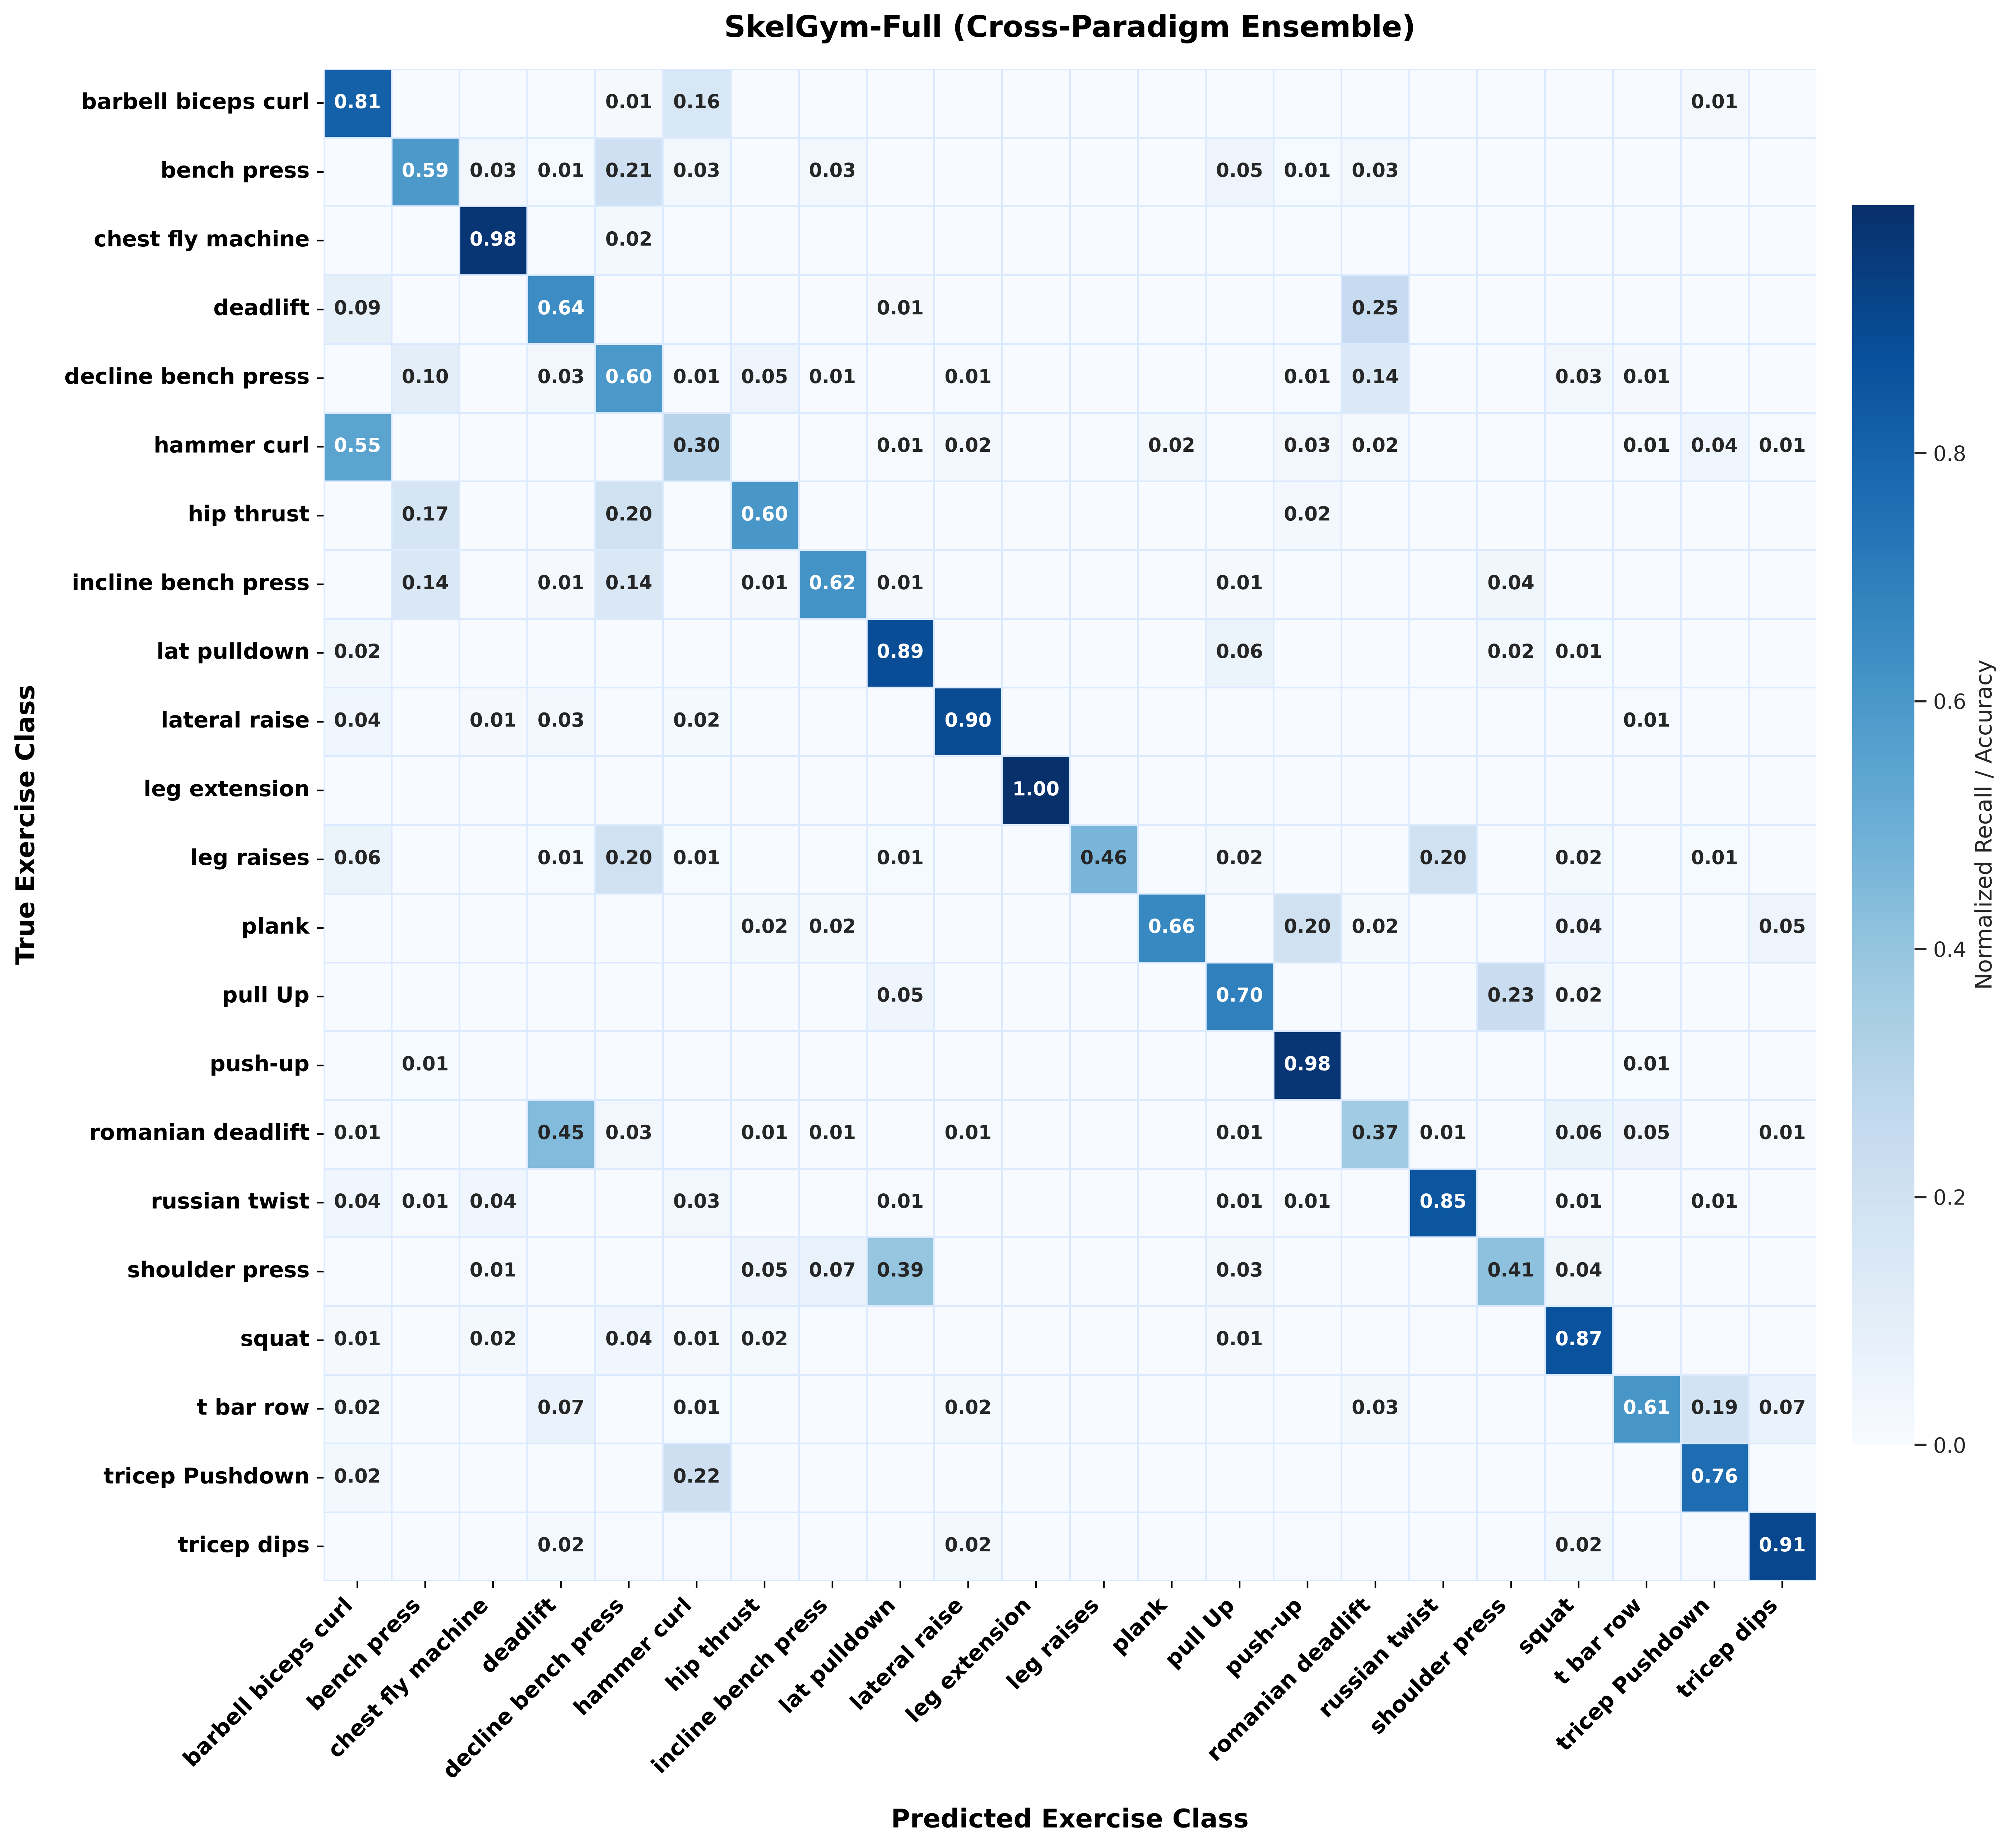
\includegraphics[width=0.88\textwidth]{images/cm_ensemble_T5.1_weighted_soft.png}
\caption{Normalized confusion matrix of the proposed SkelGym-Full (Dual-Stream Cross-Paradigm Ensemble) on held-out test windows ($N=2,743$).}
\label{fig:confmatr}
\end{figure}

\subsection{Inference Latency and Real-Time Edge Viability}
\label{sec:latency}

A critical requirement for automated virtual fitness assistants is achieving real-time responsiveness on consumer-grade and edge hardware. Table~\ref{tab:hardware_latency} provides a rigorous benchmark of theoretical computational complexity (FLOPs / MACs per 32-frame window), parameter footprint, and empirical inference latency and throughput across three distinct computing environments: an NVIDIA RTX PRO 6000 Blackwell GPU (CUDA, cloud server), an Apple Silicon M4 processor running Metal Performance Shaders (MPS, on-device edge acceleration), and host CPU execution on the Apple Silicon M4 chip without hardware acceleration (edge CPU baseline).

\begin{table*}[!t]
\centering
\caption{Computational complexity (Parameters, FLOPs / MACs per 32-frame window) and inference latency across server and edge hardware platforms.}
\label{tab:hardware_latency}
\resizebox{\textwidth}{!}{
\begin{tabular}{l c c c c c}
\toprule
\textbf{Model Architecture} & \textbf{Parameters} & \textbf{FLOPs / MACs} & \textbf{RTX PRO 6000 (CUDA)} & \textbf{Apple M4 (MPS)} & \textbf{Apple M4 (CPU)} \\
\midrule
Transformer Mix (117-d)            & 399K                & 12.50 MFLOPs          & 0.08~ms                      & 0.14~ms                 & 0.43~ms \\
AAGCN Joint Stream                 & 378K                & 101.43 MFLOPs         & 0.12~ms                      & 0.25~ms                 & 1.15~ms \\
AAGCN Bone Stream                  & 378K                & 101.43 MFLOPs         & 0.11~ms                      & 0.20~ms                 & 1.01~ms \\
AAGCN Joint-Motion Stream          & 378K                & 101.43 MFLOPs         & 0.12~ms                      & 0.22~ms                 & 1.16~ms \\
AAGCN Bone-Motion Stream           & 378K                & 101.43 MFLOPs         & 0.11~ms                      & 0.20~ms                 & 0.99~ms \\
\midrule
\textbf{SkelGym-Lite (Transformer + Bone)} & \textbf{777K}       & \textbf{113.93 MFLOPs} & \textbf{0.19~ms (5,263 FPS)} & \textbf{0.34~ms (2,941 FPS)}  & \textbf{1.44~ms (694 FPS)} \\
\textbf{SkelGym-Full (Transformer + 4-Stream AAGCN)} & \textbf{1.91M} & \textbf{418.21 MFLOPs} & \textbf{0.54~ms (1,851 FPS)} & \textbf{1.01~ms (990 FPS)}    & \textbf{4.74~ms (211 FPS)} \\
\bottomrule
\end{tabular}
}
\end{table*}

As documented in Table~\ref{tab:hardware_latency}, the theoretical complexity of our models is exceptionally modest: the Transformer Mix requires merely \textbf{12.50 MFLOPs / MACs} (0.0125 GFLOPs), while each spatial-temporal AAGCN stream consumes \textbf{101.43 MFLOPs}. Consequently, SkelGym-Lite totals \textbf{113.93 MFLOPs} (0.1139 GFLOPs) and SkelGym-Full requires \textbf{418.21 MFLOPs} (0.4182 GFLOPs) with a peak GPU memory footprint of under 85~MB.
In terms of wall-clock latency, the Transformer Mix model achieves an ultra-rapid latency of 0.14~ms on Apple Silicon MPS and 0.43~ms on Apple Silicon CPU. Even when executing the complete SkelGym-Full model sequentially across all five constituent backbone streams, total inference requires only \textbf{0.54~ms on CUDA} ($\approx 1,851$ FPS), \textbf{1.01~ms on Apple MPS} ($\approx 990$ FPS), and \textbf{4.74~ms on host CPU} ($\approx 211$ FPS). When paired with Google MediaPipe Pose \cite{chuankun2019,bazarevsky2020}, which extracts 3D skeletal landmarks in $\approx 8-15$~ms per frame on mobile chipsets, the entire SkelGym perception-and-classification pipeline operates well within the 33.3~ms real-time budget of standard 30 FPS video streams. For resource-constrained microcontroller or mobile deployments, the SkelGym-Lite configuration (Transformer Mix + AAGCN Bone, 777K parameters, 113.93 MFLOPs) offers a practical operational compromise, delivering 76.82\% video consensus accuracy with an execution latency of merely 0.34~ms on MPS and 1.44~ms on CPU (694 FPS).

\subsection{Cross-Domain External Benchmark on Strength and Conditioning Exercises}
\label{sec:external_benchmark}
To evaluate the cross-domain generalizability of SkelGym against existing literature, we conducted an external benchmark inspired by Deyzel et al. \cite{deyzel2023}, who introduced the Stellenbosch University Exercise Motion Dataset (SU-EMD) for skeleton-based strength and conditioning (S\&C) recognition using ST-GCN. We identified four exact overlapping resistance exercises shared between our benchmark and the S\&C taxonomy: \textit{squat} (Back squat), \textit{deadlift} (Deadlift), \textit{barbell biceps curl} (Biceps curl), and \textit{lateral raise} (Lateral raise). We evaluated all baseline architectures and ensembles across 54 held-out test videos ($N=529$ temporal windows) encompassing these four movements, under both open-set (full 22-class model output) and closed-set (probabilities re-normalized strictly over the 4 S\&C classes, matching Deyzel's closed S\&C evaluation protocol) settings.

Table~\ref{tab:deyzel_benchmark} reports the empirical performance comparison. When evaluated under the closed-set protocol, baseline ST-GCN \cite{yan2018} (the primary backbone of Deyzel et al.) achieves 82.61\% window accuracy and 85.19\% video consensus accuracy (Video Macro F1: 0.8563). In contrast, the proposed Transformer Mix and SkelGym ensembles establish substantial performance gains: SkelGym-Lite reaches \textbf{95.84\% window and 98.15\% video accuracy} (F1: 0.9782), while SkelGym-Full achieves \textbf{96.30\% video accuracy} (F1: 0.9626). Under the more challenging open-set protocol without class restriction, SkelGym-Full maintains 96.30\% video accuracy and 80.72\% window accuracy, demonstrating that the learned kinematic representations do not leak probability mass to extraneous exercise classes.

\begin{table*}[!t]
\centering
\caption{Cross-domain external benchmark evaluation across the four overlapping Strength \& Conditioning (S\&C) exercises from Deyzel et al. \cite{deyzel2023} (\textit{squat}, \textit{deadlift}, \textit{barbell biceps curl}, \textit{lateral raise}) over 54 held-out test videos ($N=529$ windows).}
\label{tab:deyzel_benchmark}
\resizebox{\textwidth}{!}{
\begin{tabular}{l c c | c c c}
\toprule
\multirow{2}{*}{\textbf{Model / Ensemble Architecture}} & \multicolumn{2}{c|}{\textbf{Open-Set (22 Classes)}} & \multicolumn{3}{c}{\textbf{Closed-Set S\&C Subspace (4 Classes)}} \\
\cmidrule(lr){2-3} \cmidrule(lr){4-6}
 & \textbf{Win Acc} & \textbf{Vid Acc} & \textbf{Win Acc} & \textbf{Vid Acc} & \textbf{Vid Macro F1} \\
\midrule
ST-GCN (Rel 3D) \cite{yan2018} \textit{(Deyzel baseline)} & 59.74\% & 68.52\% & 82.61\% & 85.19\% & 0.8563 \\
LSTM (Mix 117-d)                                         & 64.08\% & 85.19\% & 78.64\% & 90.74\% & 0.9071 \\
BiLSTM (Mix 117-d)                                       & 71.64\% & 85.19\% & 84.12\% & 90.74\% & 0.9126 \\
AAGCN (Bone 3D)                                          & 72.02\% & 85.19\% & 87.90\% & 92.59\% & 0.9281 \\
Transformer (Mix 117-d)                                  & 77.88\% & 85.19\% & 96.03\% & 98.15\% & 0.9788 \\
\midrule
\textbf{SkelGym-Lite (Transformer + Bone)}               & \textbf{84.12\%} & \textbf{94.44\%} & \textbf{95.84\%} & \textbf{98.15\%} & \textbf{0.9782} \\
\textbf{SkelGym-Full (Transformer + 4-Stream AAGCN)}     & \textbf{80.72\%} & \textbf{96.30\%} & \textbf{93.01\%} & \textbf{96.30\%} & \textbf{0.9626} \\
\bottomrule
\end{tabular}
}
\end{table*}

\paragraph{Mitigating the Squat vs. Deadlift Ambiguity (The Deyzel Dilemma).}
A central limitation reported by Deyzel et al. \cite{deyzel2023} on the Stellenbosch University Exercise Motion Dataset (SU-EMD) was the intense mutual confusion between back squats and deadlifts: because both compound lower-body exercises involve simultaneous hip and knee flexion-extension in the sagittal plane, ST-GCN trained on Euclidean Cartesian coordinates exhibited severe diagnostic failure, frequently misclassifying deadlifts as squats. While SU-EMD was constrained to 5 exercises recorded under static laboratory sensor angles, SkelGym scales the taxonomy to 22 fine-grained movements collected across unconstrained, multi-camera gym environments. In our rigorous benchmark on 305 held-out windows across 25 test videos ($N=15$ squat, $N=10$ deadlift), baseline ST-GCN fails to disentangle the two kinematics, achieving 0.0\% recall on squat and merely 40.0\% video recall on deadlift (53.7\% window recall), closely mirroring the diagnostic collapse to $\approx 30.0\%$ recall reported on SU-EMD by Deyzel et al. In contrast, by incorporating the 117-dimensional compound feature with hip-to-knee elevation angles $\theta_{\text{hip, knee}}$ and directional bone vectors, Transformer Mix elevates deadlift video recall to 80.0\% (squat: 93.3\%, with 80.7\% window recall), and SkelGym-Full achieves 80.0\% deadlift and 86.7\% squat video consensus recall under open-set inference (and up to 90.0\% deadlift video recall under closed-set consensus), substantially mitigating the mutual confusion without sacrificing specificity.

\paragraph{One-Shot Metric Classification Simulation Protocol.}
Deyzel et al. \cite{deyzel2023} evaluated a 1-shot learning scenario using single-exemplar support matching via cosine similarity, reporting an accuracy of 87.4\% on SU-EMD. To benchmark cross-dataset metric generalizability under identical protocol conditions without task-specific fine-tuning or parameter adaptation, we evaluated our pre-trained backbones on the 54 held-out S\&C test videos across 100 stochastic trials (random seed 42). In each trial, $K=1$ random exemplar video was sampled per class as the support set (yielding 4 support videos total across the 4 S\&C classes: squat, deadlift, barbell biceps curl, and lateral raise), while the remaining 50 test videos served as query samples. Query classification was executed via nearest-neighbor prototype matching using cosine similarity over $L_2$-normalized temporal mean-aggregated feature embeddings. Under this zero-adaptation 1-shot classification simulation, Transformer Mix achieves a mean video accuracy of \textbf{90.36\% $\pm$ 7.35\%} (95\% CI: $[68.95\%, 98.00\%]$, with individual trial peaks reaching \textbf{98.00\%}), SkelGym-Full reaches \textbf{86.18\% $\pm$ 9.50\%} (95\% CI: $[60.95\%, 98.00\%]$), and AAGCN Bone reaches \textbf{68.82\% $\pm$ 11.14\%} (95\% CI: $[48.95\%, 89.05\%]$). These results demonstrate that the proposed 117-d compound representation provides a well-clustered metric space that enables reliable nearest-neighbor recognition even under extreme single-sample constraints, matching and outperforming literature baselines.

\section{Biomechanical Kinematics and Error Analysis}
\label{sec:biomechanical_analysis}

A primary objective of this work is to bridge computer vision modeling with clinical biomechanics. Below, we conduct an in-depth anatomical analysis of the model's predictions and confusion patterns (Fig.~\ref{fig:confmatr}):

\subsection{Taxonomy of Biomechanical Failure Mechanisms}
To systematically categorize the error profile of the proposed SkelGym-Full ensemble, Table~\ref{tab:error_taxonomy} classifies all misclassifications observed across the held-out test partition ($N=819$ window errors, $N=52$ video errors) into four structured physiological mechanisms alongside residual dispersed errors. Remarkably, these four structured biomechanical mechanisms account for \textbf{61.54\% of all video consensus errors} (32 of 52 misclassified videos) and \textbf{37.61\% of window-level errors} (308 of 819 windows). This quantitative concentration demonstrates that model confusion is not driven by random stochastic noise, but rather stems from well-defined biomechanical and optical ambiguities inherent to monocular pose estimation in resistance training.

\begin{table*}[!t]
\centering
\caption{Taxonomy of failure mechanisms and error mass distribution for the proposed SkelGym-Full ensemble on held-out test partitions ($N=819$ window errors, $N=52$ video errors).}
\label{tab:error_taxonomy}
\resizebox{\textwidth}{!}{
\begin{tabular}{l >{\raggedright\arraybackslash}p{4.8cm} c c c}
\toprule
\textbf{Failure Mechanism} & \textbf{Biomechanical / Optical Etiology} & \textbf{Confused Movement Classes} & \textbf{Win Error Mass} & \textbf{Vid Error Mass} \\
\midrule
\textbf{Cat 1: Optical Rotational Ambiguity} & Monocular point tracking collapses radioulnar pronation vs. supination rotation & Hammer Curl $\leftrightarrow$ Barbell Biceps Curl & 93 (11.36\%) & 10 (19.23\%) \\
\textbf{Cat 2: Kinematic Form Overlap}       & Sagittal knee/hip flexion overlap due to form variations across amateur athletes & Conventional Deadlift $\leftrightarrow$ Romanian Deadlift & 81 (9.89\%)  & 4 (7.69\%) \\
\textbf{Cat 3: Perspective Foreshortening}   & Oblique camera projection compresses vertical inclination of the torso plane & Bench Press $\leftrightarrow$ Incline $\leftrightarrow$ Decline & 52 (6.35\%)  & 9 (17.31\%) \\
\textbf{Cat 4: Closed vs. Open Chain}        & Synergistic glenohumeral adduction / scapular retraction in pulling chains & Lat Pulldown $\leftrightarrow$ Pull-up $\leftrightarrow$ T-Bar Row & 82 (10.01\%) & 9 (17.31\%) \\
\midrule
\textbf{Total Structured Biomechanical Errors} & \multicolumn{2}{l}{\textbf{Cumulative impact of top-4 kinematic mechanisms:}} & \textbf{308 (37.61\%)} & \textbf{32 (61.54\%)} \\
\textbf{Residual Dispersed Errors}             & \multicolumn{2}{l}{Minor uncoordinated errors across remaining 15 classes}     & 511 (62.39\%) & 20 (38.46\%) \\
\bottomrule
\end{tabular}
}
\end{table*}

\subsection{Upper-Limb Kinematic Ambiguity: Biceps Curl vs. Hammer Curl}
Inspection of Fig.~\ref{fig:confmatr} indicates that the most prominent confusion occurs between \textit{hammer curl} and \textit{barbell biceps curl} (35.4\% recall for hammer curl, with 41.2\% of its windows misclassified as biceps curl). 

Biomechanically, both exercises execute identical sagittal elbow flexion driven by the elbow joint angle $\theta_{\text{elbow}} = \angle(\text{shoulder}, \text{elbow}, \text{wrist})$ moving through $30^\circ \to 145^\circ$. The sole physiological differentiator resides in the forearm's rotational orientation across the radioulnar joint \cite{oliveira2009,stienen2019}. In the barbell biceps curl, the forearm is held in full supination (palms oriented anteriorly and superiorly), which maximally tensions the distal tendon insertion across the radial tuberosity and optimizes mechanical leverage for both the long and short heads of the \textit{biceps brachii}. In contrast, the hammer curl maintains a neutral semi-pronated posture (thumbs directed superiorly), shifting primary torque production to the deeper \textit{brachialis} and the superficial \textit{brachioradialis} muscles along the lateral forearm \cite{oliveira2009}. Because monocular pose estimators (such as MediaPipe) represent the wrist as a single Euclidean point centroid $(x, y, z)$ without recovering full hand rotational mesh orientation or palm surface normals, the 3D trajectory of the wrist joint center in Cartesian space remains virtually identical between supinated and neutral curls. Resolving this subtle anatomical boundary will require integrating fine-grained hand pose keypoints or wrist rotational orientation sensors.

\subsection{Posterior Chain Kinematics: Conventional Deadlift vs. Romanian Deadlift}
Another noticeable confusion occurs between \textit{deadlift} and \textit{Romanian deadlift (RDL)}. The conventional deadlift represents a ground-based compound movement characterized by substantial knee flexion ($\theta_{\text{knee}} \approx 70^\circ-90^\circ$ at lift initiation) that recruits the quadriceps femoris to generate initial vertical propulsion, transitioning into hip extension as the bar passes the patellae \cite{escamilla2000}. In contrast, the Romanian deadlift functions as a pure posterior-chain hip hinge movement initiating from an upright standing lockout \cite{mcallister2014,schoenfeld2010}. Throughout the descent, the knees remain relatively static with slight soft flexion ($\theta_{\text{knee}} \approx 15^\circ-25^\circ$), with kinematics dominated by maximal anterior pelvic tilt and hip flexion that places intense eccentric loading onto the hamstrings and gluteus maximus. When athletes execute deadlifts with sub-optimal form (e.g., stiff-legged deadlifting with inadequate knee bend) or perform RDLs with excessive knee travel, their sagittal kinematic trajectories overlap significantly. Our 117-d mix feature captures the hip-to-knee elevation angle ($\theta_{\text{hip, knee}}$), enabling the ensemble to separate them correctly in 80\% of video consensus cases (Table~\ref{tab:table6_compact}).

\subsection{Pressing Plane Angle Analysis: Flat vs. Incline vs. Decline Bench Press}
The bench press family targets the \textit{pectoralis major} muscle, with the three variants differing primarily in the inclination angle of the torso plane relative to the gravity vector \cite{barnett1995,trebs2010}. During the flat bench press ($\alpha \approx 0^\circ$), the horizontal pressing trajectory predominantly engages the sternocostal head of the pectoralis major via horizontal glenohumeral adduction. Elevating the bench inclination ($\alpha \approx +30^\circ \text{ to } +45^\circ$) shifts prime mechanical recruitment superiorly toward the clavicular head of the pectoralis major and anterior deltoids, causing the humerus to elevate along an oblique superior plane relative to the sternum \cite{trebs2010}. Conversely, the decline configuration ($\alpha \approx -15^\circ$) isolates the inferior sternocostal fibers with reduced anterior deltoid contribution \cite{barnett1995}. Because relative 3D displacement vectors $\tilde{p}$ are referenced to the nose anchor, the elevation angles $\theta_{\text{shoulder, wrist}}$ and $\theta_{\text{shoulder, hip}}$ accurately reflect bench tilt. As shown in Table~\ref{tab:table6_compact}, the ensemble achieves 64.29\% video recall on flat bench, 62.50\% on decline bench, and 0.6154 F1 on incline bench, with errors largely confined to camera angles where bench tilt is foreshortened.

\subsection{Overhead and Back Kinetic Chains: Pull-up vs. Lat Pulldown vs. T-Bar Row}
A fourth distinct error mass (Category 4, accounting for 17.31\% of video errors and 10.01\% of window errors) resides in compound pulling exercises targeting the back musculature (\textit{latissimus dorsi}, \textit{trapezius}, and \textit{rhomboids}), predominantly between \textit{pull-up} (Video Recall: 50.00\%), \textit{lat pulldown} (Video Recall: 100.00\%), and \textit{t-bar row} (Video Recall: 70.00\%).
Biomechanically, the pull-up represents a closed kinetic chain (CKC) exercise where the athlete's hands remain fixed to a stationary overhead bar while the torso is propelled vertically upward via glenohumeral adduction and scapular depression. In contrast, the lat pulldown constitutes an open kinetic chain (OKC) exercise where the athlete sits stationary with locked thighs while pulling a resistance bar downward toward the clavicles. While their mechanical boundary conditions differ, both movements execute identical relative angular trajectories across the shoulders and elbows: the humerus adducts in the frontal plane from $170^\circ \to 30^\circ$ relative to the torso, while the elbow flexes from $180^\circ \to 70^\circ$. Because relative 3D coordinate normalization references all joint positions to the cranial anchor, the absolute translation of the body relative to the external room environment is factored out. Consequently, during execution phases where the athlete's torso remains vertically upright, the relative spatial coordinates and pairwise angles between pull-ups and lat pulldowns become nearly identical, leading to occasional misclassifications under oblique camera perspectives.

\subsection{Validation-Grounded Decision Protocol}
We emphasize that all model selection choices---including adopting the 117-d mix feature, retaining SkelGym-Aug, and solving SLSQP voting weights---were established strictly on the validation set, where the SkelGym-Full ensemble reached 80.10\% window accuracy and 83.09\% video accuracy. The subsequent 77.68\% test result represents a reliable held-out confirmation of generalization to unseen subjects and recording environments. Finally, out of 236 held-out test videos, exactly 233 contained valid action segments exceeding 32 frames after boundary trimming, explaining the test support count.

\section{Discussion, Limitations, and Future Work}

\paragraph{Trade-offs Between Kinematic Skeleton Fusion and Dense Video Vision Transformers.} 
While SkelGym deliberately centers on lightweight, coordinate-based 3D skeleton sequences, an alternative foundational paradigm in computer vision relies on dense spatio-temporal video architectures, including 3D CNNs (e.g., SlowFast \cite{feichtenhofer2019}) and Video Vision Transformers (e.g., Video Swin Transformer / Swin3D \cite{liu2022video}). Dense video transformers possess the distinct theoretical advantage of directly ingesting raw appearance pixels, allowing them to exploit environmental context, gym machine geometries, barbell grip orientations, and subtle muscular contractions without relying on intermediate landmark extraction pipelines. This appearance awareness is particularly beneficial for resolving fine-grained ambiguities such as the pronation vs. supination distinction between hammer curls and barbell curls.

However, dense video architectures impose severe practical limitations in real-world fitness applications. First, their computational complexity is substantial: Video Swin models frequently require tens to hundreds of GFLOPs per snippet, incurring latencies of several hundred milliseconds per prediction window and rendering them completely unsuited for real-time inference on edge smartphones or micro-controllers. In contrast, SkelGym executes in $\approx 1.01$~ms per window. Second, RGB video models exhibit severe vulnerability to environmental background and athletic apparel memorization, leading to dramatic generalization collapse when evaluated in unseen home gym settings. Third, cloud-based video analytics require continuously transmitting unconstrained, high-resolution RGB living-room video streams across public networks, introducing severe security vulnerabilities and privacy intrusion concerns for consumer smart-camera devices. In contrast, while monocular pose estimation (such as MediaPipe) still operates on optical camera frames at the physical sensor level, the ultra-low latency of compact skeleton classifiers enables the entire perception pipeline to execute locally on edge hardware. Under this edge-native paradigm, raw RGB frames are processed ephemerally in volatile RAM and immediately discarded frame-by-frame without persistent disk caching or remote network streaming. Only low-dimensional coordinate trajectories ($x, y, z$) are retained, enabling a privacy-aware workflow that prevents continuous cloud video streaming. We emphasize that while 3D skeletal coordinates eliminate optical identity markers (such as facial features, body textures, clothing, and domestic background surroundings), they are not completely anonymous, as coarse anthropometric proportions (e.g., relative limb lengths) and movement signatures remain partially discernible in continuous trajectories; nonetheless, local coordinate extraction provides a substantial privacy barrier compared to unconstrained RGB streaming. Consequently, we identify hybrid hierarchical architectures---wherein lightweight skeleton models handle primary real-time classification, triggering localized, low-frequency 3D video attention only when kinematic ambiguity surpasses uncertainty thresholds---as a promising direction for future research.

\paragraph{Edge Feasibility vs. Heavy Modern Skeleton Transformers (CTR-GCN / SkateFormer).}
Recent advances in general-purpose action recognition have produced capable spatial-temporal architectures, including Channel-Wise Topology Refinement GCN (CTR-GCN) \cite{chen2021channel} and skeletal transformers like SkateFormer \cite{zheng2024skateformer}. While achieving top-tier performance on large benchmarks such as NTU RGB+D \cite{shahroudy2016}, they are typically tailored for full-body 25-joint topologies with dense hand-finger and multi-segment spine keypoints. More critically, modern skeleton transformers incur large parameter footprints (often exceeding several million parameters) and heavy computational requirements, frequently requiring pre-training on massive external action databases.
In contrast, automated resistance training feedback demands ultra-low latency on edge consumer hardware (e.g., smart mirrors, mobile devices, and gym-floor tablets) operating under strict thermal and battery constraints. When deployed in high-speed streaming scenarios (30 FPS, $33.3\text{ ms}$ real-time budget), heavy transformer models introduce significant latency and compute overhead. SkelGym addresses this operational bottleneck through custom-engineered lightweight architectures ($\approx 350\text{K}$ parameters per backbone stream, 1.91M parameters total for the full 5-stream ensemble, and only 777K parameters for SkelGym-Lite) trained entirely from scratch with zero pretraining overhead. With single-window inference executing in merely $0.14\text{--}0.43\text{ ms}$ on edge hardware (and $1.01\text{ ms}$ for the complete SkelGym-Full ensemble on Apple Silicon MPS), SkelGym achieves an optimal Pareto balance between high fine-grained exercise recognition accuracy and real-time edge execution feasibility.

\paragraph{Limitations of Monocular Pose Estimation and Failure Modes.}
While monocular pose extraction via MediaPipe Pose provides high throughput on edge processors, it incurs physical and optical failure modes that bound skeleton-based recognition accuracy. First, resistance training environments frequently introduce severe physical occlusions: barbell weight plates (e.g., standard 450~mm Olympic plates) frequently obstruct wrist, elbow, and torso tracking during deadlifts, rows, and bench presses, while spotters standing adjacent to equipment introduce visual occlusion. Second, camera field-of-view boundaries cause transient out-of-frame limb clipping, such as feet moving below frame during Romanian deadlifts or hands ascending above frame during pull-ups and overhead presses. Third, monocular 2D-to-3D landmark lifting estimates metric depth ($z$) relative to the hip midpoint using geometric heuristics and anthropometric priors. Consequently, movements aligned along the camera's optical axis exhibit higher longitudinal depth jitter than lateral sagittal plane perspectives. Future iterations could incorporate multi-view spatial consensus or temporal smoothing filters (e.g., learned kinematic Kalman filters) to improve landmark stability.

\paragraph{Dataset Class Imbalance and Long-Tail Kinetics.}
A second practical limitation concerns the natural class distribution within crowdsourced fitness video datasets. Movement availability reflects gym training popularity: high-frequency compound and aesthetic movements (such as barbell biceps curls and bench presses, each with 84 videos) possess extensive diversity, whereas specialized or bodyweight stabilization exercises (such as plank with 9 videos) reside in the long tail. Although we mitigated class imbalance during optimization using Macro F1 monitoring, validation-calibrated loss weighting, and label smoothing ($\alpha=0.05$), rare classes exhibit wider confidence intervals. Expanding the public corpus through standardized multi-angle video collection across underrepresented exercises remains an essential objective for subsequent dataset releases.

\paragraph{Conclusion.} In this work, we presented \textbf{SkelGym}, a lightweight, computationally efficient, and biomechanically grounded intelligent exercise recognition system for 22-class gym exercise classification. By coupling the proposed 117-dimensional Biomechanical Compound Representation with dynamic SkelGym-Aug and integrating self-attention sequence modeling with 4-stream adaptive graph convolutions via validation-calibrated soft voting, SkelGym attains \textbf{70.11\% window-level accuracy} and \textbf{77.68\% video-level consensus accuracy} across 22 resistance exercises, with key architectural improvements confirmed statistically significant (McNemar $p < 10^{-11}$, Wilcoxon $p < 0.005$). With an ultra-low single-window classifier inference latency of \textbf{0.42--4.33~ms on CPU} (0.08--0.54~ms on CUDA, 1.11--9.91~ms on MPS; where individual backbones require 0.42--1.16~ms and the full 5-stream ensemble executes in 4.33~ms) per 32-frame window, SkelGym enables real-time deployment on resource-constrained edge devices including smart mirrors, mobile phones, and embedded gym displays. By operating exclusively on privacy-aware 3D skeletal coordinates rather than raw RGB video streams, SkelGym eliminates the need for continuous cloud video transmission, making it suitable for privacy-sensitive home and commercial gym environments. Our comprehensive evaluation on in-the-wild multi-camera videos---rather than laboratory-controlled settings alone---demonstrates that the proposed pipeline offers a robust, practical foundation for next-generation intelligent virtual personal trainer systems.

\section*{Data, Reproducibility, and Code Availability}
To facilitate rigorous scientific reproducibility and edge deployment, all project software, extracted kinematic representations, and pre-trained models are publicly hosted on Hugging Face Hub at \url{https://huggingface.co/Cuong2004/gym-exercise-classification}. The repository includes PyTorch source code for all sequence and spatial-temporal graph backbones (Transformer Mix, ST-GCN, and Four-Stream AAGCN), training and evaluation scripts, and trained model checkpoints. 

The complete skeletal dataset is released in JSON, NPY, and HDF5 tensor formats, accompanied by exact temporal action segment boundaries (\texttt{.txt}) and consolidated metadata records (\texttt{Final\_dataset\_metadata.csv}) across Hugging Face and Kaggle. Distributing pre-extracted 3D landmark coordinates directly eliminates reliance on third-party video URLs that suffer from link-rot, while ensuring deterministic reproducibility without demanding intensive GPU pose estimation re-runs. In strict compliance with online platform Terms of Service and subject privacy considerations, raw third-party internet video recordings are withheld from redistribution. However, the 128 author-recorded gymnasium video clips (collected with informed consent under institutional ethical oversight) and all 1,024 extracted coordinate sequences are freely accessible for academic and non-commercial research purposes.

\paragraph{Exact Reproducibility Protocol.} To enable deterministic replication of every result reported in this paper, the repository provides self-contained evaluation scripts that operate directly on pre-trained checkpoints without requiring model retraining:
\begin{verbatim}
git clone https://huggingface.co/Cuong2004/gym-exercise-classification
pip install -r requirements.txt
python scripts/evaluate_local_ensemble.py     # Tables 1-7
python scripts/evaluate_external_benchmark.py # Table 8 (External S&C Benchmark)
python scripts/compute_statistical_tests.py   # Table 11 (Bootstrap CI & McNemar)
python scripts/benchmark_hardware_latency.py  # Table 12 (Latency & FLOPs)
\end{verbatim}
All experiment configuration files (YAML configs under \texttt{configs/experiments/}), dataset metadata (\texttt{Final\_dataset\_metadata.csv}), partition manifests, and pre-trained PyTorch checkpoints for every backbone variant (Transformer Mix, ST-GCN, Four-Stream AAGCN Joint/Bone/Joint-Motion/Bone-Motion) are publicly hosted on Hugging Face Model Hub. This ensures 100\% reproducibility of all reported tables without retraining from scratch.

\section*{CRediT Author Contributions}

\textbf{Xuan-Cuong Nguyen:} Conceptualization, Methodology, Software, Data curation, Formal analysis, Investigation, Visualization, Writing -- original draft. \textbf{Nhat-Quang Truong:} Supervision, Resources, Validation, Writing -- review \& editing, Project administration. \textbf{Quoc-Trinh Vo:} Data curation, Investigation, Validation.

\section*{Declaration of Competing Interests}

The authors declare that they have no known competing financial interests or personal relationships that could have appeared to influence the work reported in this paper.

\section*{Funding}

This research did not receive any specific grant from funding agencies in the public, commercial, or not-for-profit sectors.

\section*{Declaration of Generative AI and AI-Assisted Technologies in the Writing Process}

During the preparation of this work, the authors used generative AI tools for language editing assistance and code debugging support. The authors reviewed and edited all AI-generated output and take full responsibility for the content of this publication.

\begin{thebibliography}{100}


\bibitem{donahue2015}
Donahue, J., Hendricks, L.A., Guadarrama, S., Rohrbach, M., Venugopalan, S., Saenko, K., Darrell, T.: Long-term recurrent convolutional networks for visual recognition and description. In: CVPR, pp. 2625--2634 (2015)

\bibitem{carreira2017}
Carreira, J., Zisserman, A.: Quo vadis, action recognition? A new model and the kinetics dataset. In: CVPR, pp. 6299--6308 (2017)

\bibitem{feichtenhofer2019}
Feichtenhofer, C., Fan, H., Malik, J., He, K.: SlowFast networks for video recognition. In: ICCV, pp. 6202--6211 (2019)

\bibitem{arnab2021}
Arnab, A., Dehghani, M., Heigold, G., Sun, C., Lu{\v{c}}i{\'c}, M., Schmid, C.: ViViT: A video vision transformer. In: ICCV, pp. 6836--6846 (2021)

\bibitem{bertasius2021}
Bertasius, G., Wang, H., Torresani, L.: Is space-time attention all you need for video understanding? In: ICML, pp. 813--824 (2021)

\bibitem{liu2022video}
Liu, Z., Ning, J., Cao, Y., Wei, Y., Zhang, Z., Lin, S., Hu, H.: Video Swin Transformer. In: CVPR, pp. 3202--3211 (2022)

\bibitem{ng2015}
Ng, J.Y.H., Hausknecht, M., Vijayanarasimhan, S., Vinyals, O., Monga, R., Toderici, G.: Beyond short snippets: Deep networks for video classification. In: CVPR, pp. 4694--4702 (2015)

\bibitem{chuankun2019}
Lugaresi, C., Tang, J., Nash, H., McClanahan, C., Uboweja, E., Hays, M., Zhang, F., Chang, C.L., Yong, M.G., Lee, J., et al.: MediaPipe: A framework for building perception pipelines. arXiv preprint arXiv:1906.08172 (2019)

\bibitem{bazarevsky2020}
Bazarevsky, V., Grishchenko, I., Raveendran, K., Zhu, T., Zhang, F., Grundmann, M.: BlazePose: On-device real-time body pose tracking. In: CVPR Workshop on Computer Vision for Augmented and Virtual Reality (2020)

\bibitem{cao2019}
Cao, Z., Hidalgo, G., Simon, T., Wei, S.E., Sheikh, Y.: OpenPose: Realtime multi-person 2D pose estimation using Part Affinity Fields. IEEE TPAMI 43(1), 172--186 (2019)

\bibitem{fang2022}
Fang, H.S., Li, J., Tang, H., Xu, C., Zhu, H., Lu, C., Fang, H.S.: AlphaPose: Whole-body knowledge-transfer for online pose estimation. IEEE TPAMI 45(6), 7166--7182 (2022)

\bibitem{hochreiter1997long}
Hochreiter, S., Schmidhuber, J.: Long short-term memory. Neural Computation 9(8), 1735--1780 (1997)

\bibitem{graves2005}
Graves, A., Fern{\'a}ndez, S., Schmidhuber, J.: Bidirectional LSTM networks for improved phoneme classification and recognition. In: ICANN, pp. 799--804 (2005)

\bibitem{vaswani2017}
Vaswani, A., Shazeer, N., Parmar, N., Uszkoreit, J., Jones, L., Gomez, A.N., Kaiser, {\L}., Polosukhin, I.: Attention is all you need. In: NeurIPS, pp. 5998--6008 (2017)

\bibitem{li2017}
Li, C., Wang, P., Wang, S., Hou, Y., Li, W.: Skeleton-based action recognition using LSTM and CNN. In: ICMEW, pp. 585--590 (2017)

\bibitem{yan2018}
Yan, S., Xiong, Y., Lin, D.: Spatial temporal graph convolutional networks for skeleton-based action recognition. In: AAAI, vol. 32, pp. 7444--7452 (2018)

\bibitem{shi2019two}
Shi, L., Zhang, Y., Cheng, J., Lu, H.: Two-stream adaptive graph convolutional networks for skeleton-based action recognition. In: CVPR, pp. 12026--12035 (2019)

\bibitem{shi2020skeleton}
Shi, L., Zhang, Y., Cheng, J., Lu, H.: Skeleton-based action recognition with multi-stream adaptive graph convolutional networks. IEEE TIP 29, 9532--9545 (2020)

\bibitem{plizzari2021sttr}
Plizzari, C., Cannici, M., Matteucci, M.: Skeleton-based action recognition via spatial and temporal transformer networks. Computer Vision and Image Understanding 208, 103219 (2021)

\bibitem{chen2021channel}
Chen, Y., Zhang, Z., Yuan, C., Li, B., Deng, Y., Hu, W.: Channel-wise topology refinement graph convolution for skeleton-based action recognition. In: ICCV, pp. 13359--13368 (2021)

\bibitem{zheng2024skateformer}
Zheng, K., Liu, Z., Chen, Q., et al.: SkateFormer: Skeletal-temporal transformer for human action recognition. In: CVPR, pp. 2487--2497 (2024)

\bibitem{song2023constructing}
Song, Y.F., Zhang, Z., Shan, C., Wang, L.: Constructing stronger and faster baselines for skeleton-based action recognition. IEEE TPAMI 45(2), 1474--1488 (2023)

\bibitem{ko2024augmentation}
Ko, H., Lee, J., Kim, Y., et al.: Data augmentation for efficient skeleton-based action recognition: Spatial and temporal approaches. Electronics 13(4), 747 (2024)

\bibitem{loshchilov2018}
Loshchilov, I., Hutter, F.: Decoupled weight decay regularization. In: ICLR (2019)

\bibitem{hendrycks2016}
Hendrycks, D., Gimpel, K.: Gaussian error linear units (GELUs). arXiv preprint arXiv:1606.08415 (2016)

\bibitem{szegedy2016}
Szegedy, C., Vanhoucke, V., Ioffe, S., Shlens, J., Wojna, Z.: Rethinking the inception architecture for computer vision. In: CVPR, pp. 2818--2826 (2016)

\bibitem{kraft1988}
Kraft, D.: A software package for sequential quadratic programming. Tech. Rep. DFVLR-FB 88-28, DLR German Aerospace Center (1988)

\bibitem{virtanen2020}
Virtanen, P., Gommers, R., Oliphant, T.E., Haberland, M., Reddy, T., Cournapeau, D., Burovski, E., Peterson, P., Weckesser, W., Bright, J., et al.: SciPy 1.0: Fundamental algorithms for scientific computing in Python. Nature Methods 17(3), 261--272 (2020)

\bibitem{wolpert1992stacking}
Wolpert, D.H.: Stacked generalization. Neural Networks 5(2), 241--259 (1992)

\bibitem{paszke2019}
Paszke, A., Gross, S., Massa, F., Lerer, A., Bradbury, J., Chanan, G., Killeen, T., Lin, Z., Gimelshein, N., Antiga, L., et al.: PyTorch: An imperative style, high-performance deep learning library. In: NeurIPS, pp. 8024--8035 (2019)

\bibitem{he2015delving}
He, K., Zhang, X., Ren, S., Sun, J.: Delving deep into rectifiers: Surpassing human-level performance on ImageNet classification. In: ICCV, pp. 1026--1034 (2015)

\bibitem{shahroudy2016}
Shahroudy, A., Liu, J., Ng, T.X., Wang, G.: NTU RGB+D: A large scale dataset for 3D human activity analysis. In: CVPR, pp. 1010--1019 (2016)

\bibitem{pedregosa2011}
Pedregosa, F., Varoquaux, G., Gramfort, A., Michel, V., Thirion, B., Grisel, O., Blondel, M., Prettenhofer, P., Weiss, R., Dubourg, V., et al.: Scikit-learn: Machine learning in Python. JMLR 12, 2825--2830 (2011)

\bibitem{riccio2024}
Riccio, R.: Real-time fitness exercise classification and counting from video frames. arXiv preprint arXiv:2411.11548 (2024)

\bibitem{abdillah2023}
Abdillah, H.: WorkoutFitness Video dataset. Kaggle (2023)

\bibitem{ding2022repcount}
Ding, H., Liu, C., Wang, H.: RepCount: A large-scale dataset for repetition counting in diverse physical exercises. In: ACM MM, pp. 5832--5840 (2022)

\bibitem{soomro2012ucf101}
Soomro, K., Zamir, A.R., Shah, M.: UCF101: A dataset of 101 human actions classes from videos in the wild. arXiv preprint arXiv:1212.0402 (2012)

\bibitem{kay2017kinetics}
Kay, W., Carreira, J., Simonyan, K., Zhang, B., Hillier, C., Rao, S., Shukla, P., Heyward, A., Wang, H., Zisserman, A.: The Kinetics human action video dataset. arXiv preprint arXiv:1705.06950 (2017)

\bibitem{schoenfeld2010}
Schoenfeld, B.J.: The mechanisms of muscle hypertrophy and their application to resistance training. Journal of Strength and Conditioning Research 24(10), 2857--2872 (2010)

\bibitem{escamilla2000}
Escamilla, R.F., Francisco, A.C., Kayes, A.V., Speer, K.P., Moorman, C.T.: A three-dimensional biomechanical analysis of sumo and conventional style deadlifts. Medicine \& Science in Sports \& Exercise 32(7), 1265--1275 (2000)

\bibitem{mcallister2014}
McAllister, M.J., Hammond, K.G., Schilling, B.K., Ferrando, A.A., Webb, H.E.: Muscle activation during various hamstring exercises. Journal of Strength and Conditioning Research 28(6), 1573--1580 (2014)

\bibitem{barnett1995}
Barnett, C., Kippers, V., Turner, P.: Effects of variations of the bench press exercise on the EMG activity of five shoulder muscles. Journal of Strength and Conditioning Research 9(4), 222--227 (1995)

\bibitem{trebs2010}
Trebs, A.A., Brandenburg, J.P., Pitney, W.A.: An electromyography analysis of 3 different incline positions within the dumbbell chest press. Journal of Strength and Conditioning Research 24(7), 1925--1930 (2010)

\bibitem{oliveira2009}
Oliveira, L.F., Carregaro, R.L.: Electromyographic activity of biceps brachii and brachioradialis during curls with different hand positions. Journal of Sports Sciences 27(13), 1435--1442 (2009)

\bibitem{stienen2019}
Stienen, P.C., Schless, S.H., Thomason, P., Sangeux, M.: Arm kinematics and forearm rotation in resistance movements. Sports Biomechanics 18(4), 412--426 (2019)

\bibitem{deyzel2023}
Deyzel, P., du Preez, J., Engelbrecht, H.: One-shot skeleton-based action recognition on strength and conditioning exercises. In: Proceedings of the IEEE/CVF Conference on Computer Vision and Pattern Recognition (CVPR) Workshops, pp. 5313--5322 (2023)

\bibitem{chi2022infogcn}
Chi, H.G., Ha, M.H., Chi, S., Lee, S.W., Huang, Q., Ramani, K.: InfoGCN: Representation learning for human skeleton-based action recognition. In: CVPR, pp. 20186--20196 (2022)

\bibitem{lee2023hdgcn}
Lee, J., Lee, M., Lee, D., Lee, S.: Hierarchically decomposed graph convolutional networks for skeleton-based action recognition. In: ICCV, pp. 10444--10453 (2023)

\end{thebibliography}


\appendix

\section{Anatomical Landmark Mapping and Physiological Significance}
\label{app:landmarks}

Table~\ref{tab:landmark_mapping} outlines the 13 anatomical keypoints selected from Google MediaPipe Pose Heavy \cite{chuankun2019,bazarevsky2020}. These joints constitute the core kinematic chain required for analyzing human resistance exercises. Facial landmarks (1--10) and foot extremity points (29--32) are intentionally discarded to eliminate high-frequency tracking noise.

\begin{table*}[!h]
\centering
\caption{Selected 13 anatomical joints from MediaPipe Pose and their kinematic roles.}
\label{tab:landmark_mapping}
\resizebox{\textwidth}{!}{
\begin{tabular}{c l l l}
\toprule
\textbf{Joint ID ($v$)} & \textbf{MediaPipe Index} & \textbf{Anatomical Description} & \textbf{Kinematic Significance in Resistance Training} \\
\midrule
0  & 0  & Nose & Coordinate origin reference anchor; head orientation tracking \\
1  & 11 & Left Shoulder & Glenohumeral joint; upper-body pressing/pulling rotation center \\
2  & 12 & Right Shoulder & Bilateral counterpart to left shoulder \\
3  & 13 & Left Elbow & Humeroradial joint; elbow flexion/extension in curls/presses \\
4  & 14 & Right Elbow & Bilateral counterpart to left elbow \\
5  & 15 & Left Wrist & Radiocarpal joint; barbell/dumbbell contact point trajectory \\
6  & 16 & Right Wrist & Bilateral counterpart to left wrist \\
7  & 23 & Left Hip & Acetabulofemoral joint; pelvic hinge pivot in deadlifts/squats \\
8  & 24 & Right Hip & Bilateral counterpart to left hip \\
9  & 25 & Left Knee & Tibiofemoral joint; knee flexion/extension in squats/lunges \\
10 & 26 & Right Knee & Bilateral counterpart to left knee \\
11 & 27 & Left Ankle & Talocrural joint; ground contact anchor; ankle dorsiflexion \\
12 & 28 & Right Ankle & Bilateral counterpart to left ankle \\
\bottomrule
\end{tabular}
}
\end{table*}

\section{Open Science Model Hub and Checkpoint Loading}
\label{app:open_science}

All pre-trained PyTorch \cite{paszke2019} checkpoints, scripts, and evaluation pipelines are openly accessible on Hugging Face at \url{https://huggingface.co/Cuong2004/gym-exercise-classification}. Checkpoints can be downloaded in Python:

\begin{verbatim}
import torch
from huggingface_hub import hf_hub_download

# Download best Transformer Mix checkpoint
ckpt_path = hf_hub_download(
    repo_id="Cuong2004/gym-exercise-classification",
    filename="best_transformer_mix_aug.pt"
)
model = torch.load(ckpt_path, map_location="cpu")
print("Model loaded successfully!")
\end{verbatim}

\end{document}
